\section{\texorpdfstring{Search for $\stoptwobar$ production}{Search for t2t2 production}}
\label{sec:Stop2}
This search is focused on the pair-production of supersymmetric top-quark partners, or stop quarks. The ATLAS collaboration has published several searches for stop quarks, and no significant excess was found. The exclusion limits as a function of the mass of the lighter stop quark, \stopone, and the mass of the neutralino, \neutralino, are summarized in figure~\ref{fig:ATLAS_stop}.
Although a wide range of the allowed masses was excluded, some low-mass regions remain uncovered. One of this ``gaps'' is present in the region where the mass difference between the \stopone\ and neutralino is close to the top mass: $m_{\stopone} \approx m_t + m_{\neutralino}$. The similarity in kinematics to \ttbar\ production makes this a very challenging region to explore. In this case, a higher sensitivity can be achieved searching for the heavier stop, \stoptwo, and its subsequent decay. 
Although the \xsec\ for $\stoptwobar$ is lower by definition than $\stoponebar$, the additional decay products provide very particular kinematic features and experimental handles to suppress the background.

A search is presented for $\stoptwobar$ production targeting the decay of $\stoptwo$ into a Higgs boson and 
the lighter stop: $\stoptwobar \to \stopone H \antistopone H$, and the subsequent decay $\stopone \to t\neutralino$. The \stopone\ mass is fixed to be $m_{\stopone} = m_{\neutralino} + \unit[180]{\gev}$, in order to study the region where traditional searches have little sensitivity. This leaves two masses as free parameters, $m_{\stoptwo}$ and $m_{\neutralino}$, and the branching ratio is assumed to be BR$(\stoptwo \to \stopone H) = 1$.
For the dominant $H\to b\bar{b}$ decay mode, the final state signature contains a top-antitop pair, up two four additional heavy-flavor jets and two neutralinos.
This final state produces a very peculiar signature that is rarely produced by SM processes.
A more general analysis is also performed where, for representative values of the masses of $\st_2$ and $\neut$, the three decay modes of the $\stoptwo$ are allowed: $\stoptwo \to \stopone H$, $\stopone Z$, $t\neutralino$.

\begin{figure}[tbp!]
  \centering
  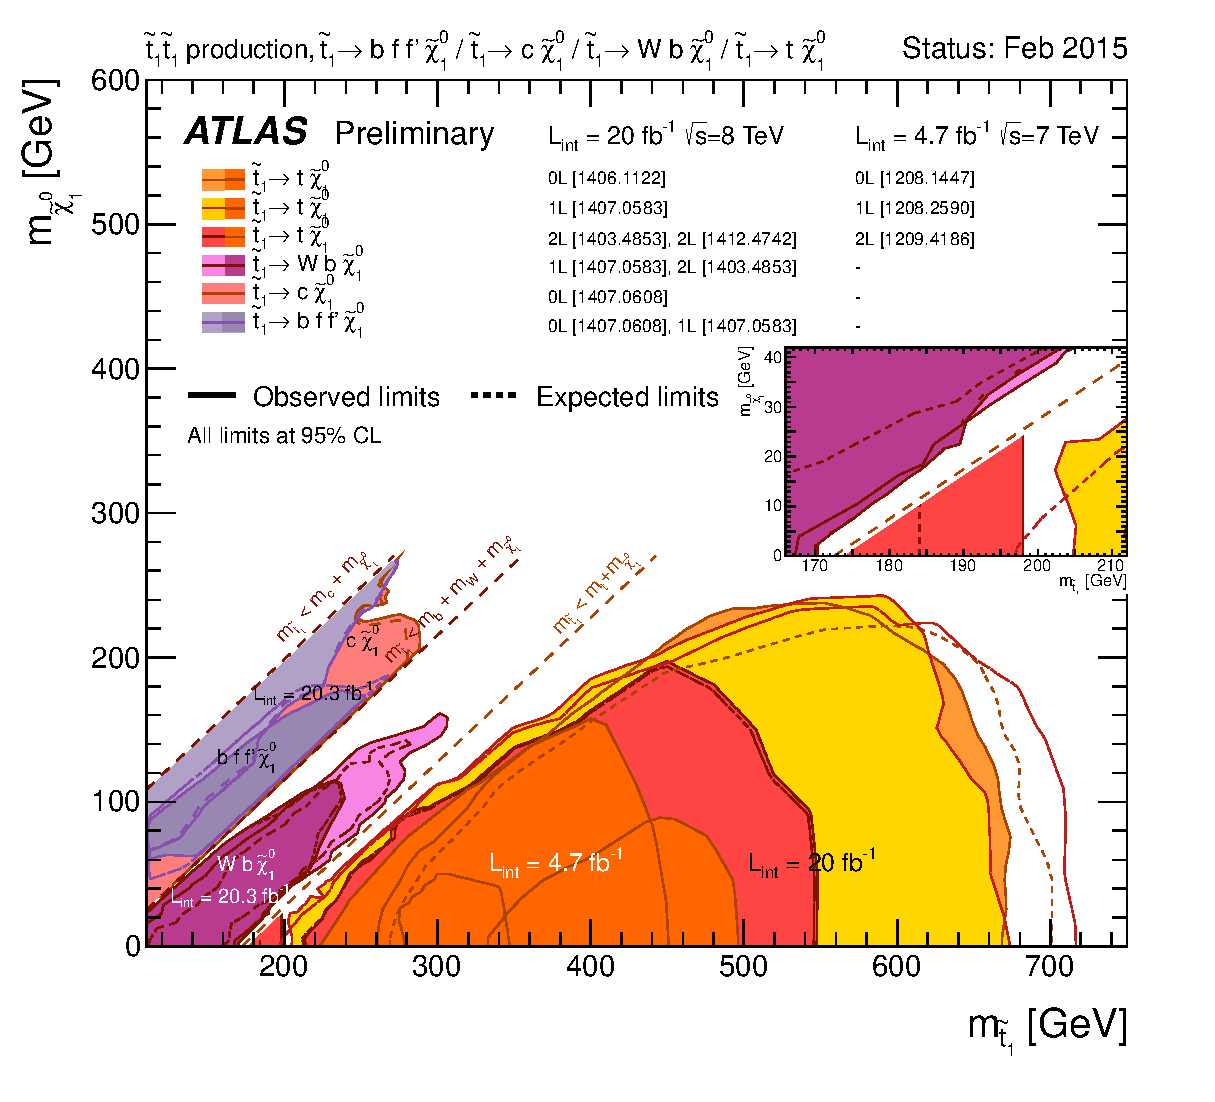
\includegraphics[width=0.7\textwidth]{Analysis/Figures_stop2/ATLAS_SUSY_Stop_tLSP.eps}
  \caption{Summary of the dedicated ATLAS searches for stop quark pair production based on $\unit[20]{fb^{-1}}$ of \pp\ collision data taken at $\sqrt{s} = \unit[8]{\tev}$, and  $\unit[4.7]{fb^{-1}}$ of \pp\ collision data taken at $\sqrt{s} = \unit[7]{\tev}$. Exclusion limits at \unit[95]{\%} CL are shown in the $\stopone-\neutralino$ mass plane. 
The dashed and solid lines show the expected and observed limits, respectively, including all uncertainties except the theoretical signal \xsec\ uncertainty (PDF and scale).
The region targeted by this analysis corresponds to the rightmost diagonal, corresponding to $m_{\stopone} \approx m_t + m_{\neutralino}$.
}
  \label{fig:ATLAS_stop}
\end{figure}

\subsection{Event selection and categorization}

Figure~\ref{fig:shapestop_njet} compares the jet multiplicity distribution
after preselection between the total background and the signal for different masses of the \stoptwo\ and \neutralino.
Signal events have, on average, higher jet multiplicity than the background.   
The presence of up to two Higgs bosons in the final state which decay dominantly to a \bbbar\ pair results in a higher $b$-tag multiplicity 
than for the background, as illustrated in figure~\ref{fig:shapestop_nbtag} for events with $\geq$6 jets.

\begin{figure}[!btp]
\centering
\begin{subfigure}{0.49\textwidth}{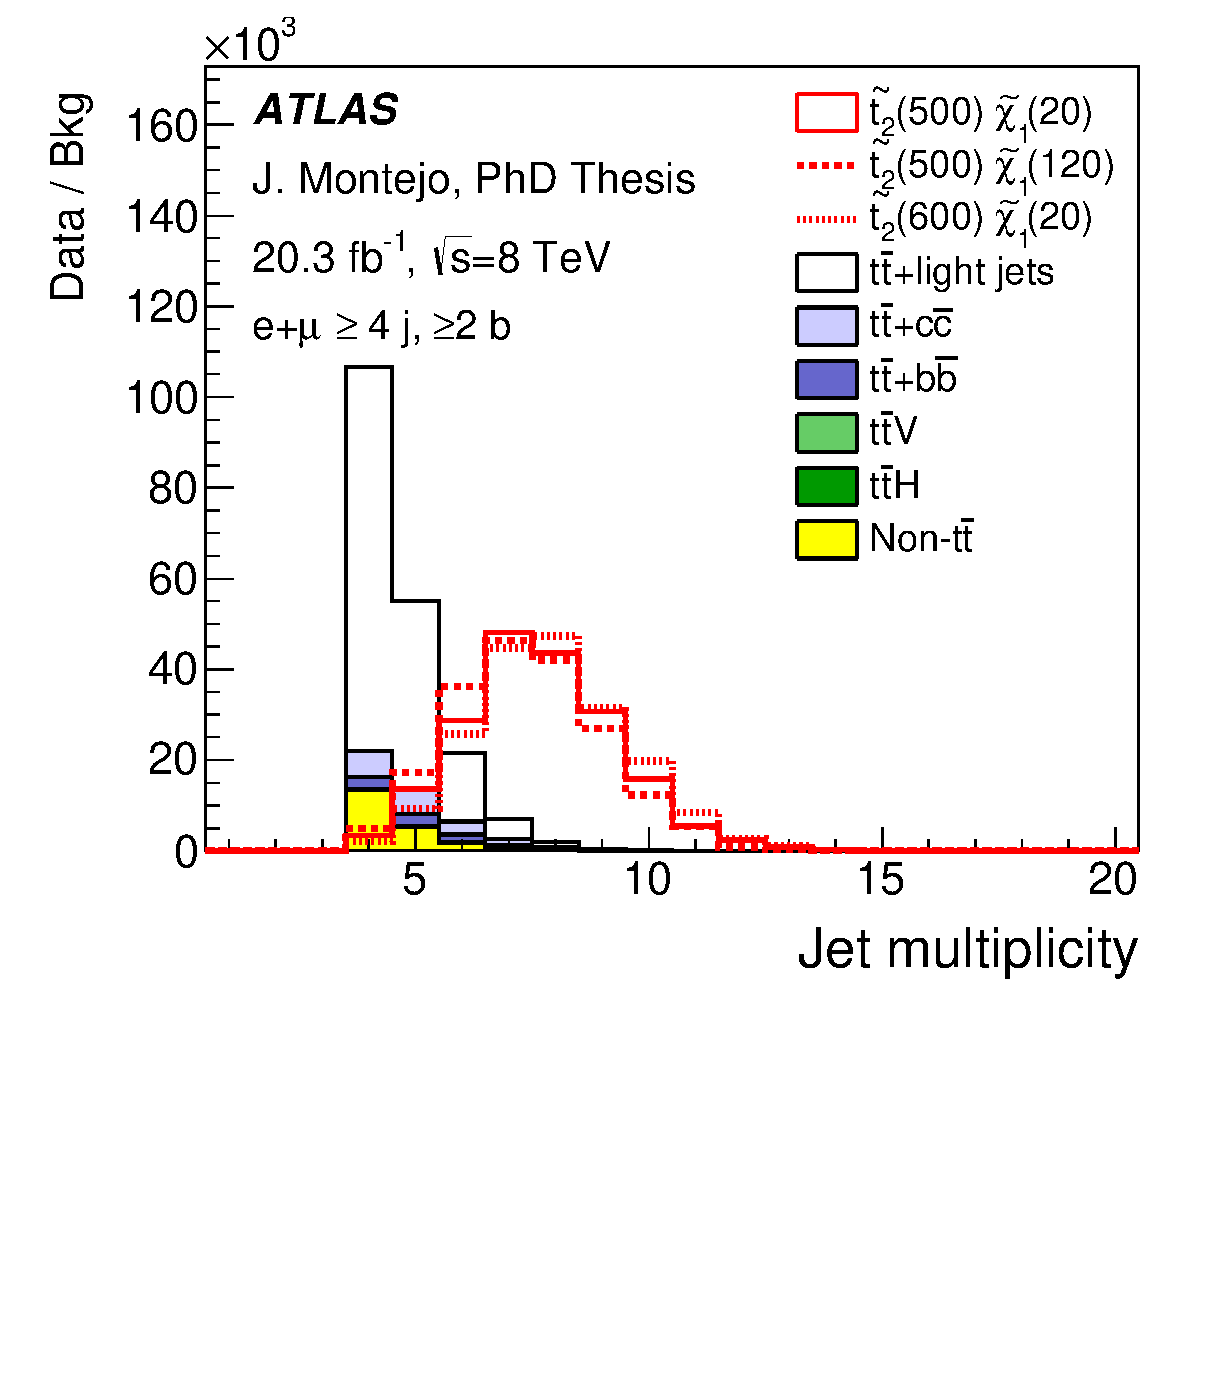
\includegraphics[trim=0cm 5cm 0cm 0cm, clip=true, width=\textwidth]{Analysis/Figures_stop2/plots_stop2/ELEMUON/4jetin/2btagin/jet_n_ELEMUON_4jetin2btagin_NOMINAL}}\caption{}\label{fig:shapestop_njet}
    \end{subfigure}
\begin{subfigure}{0.49\textwidth}{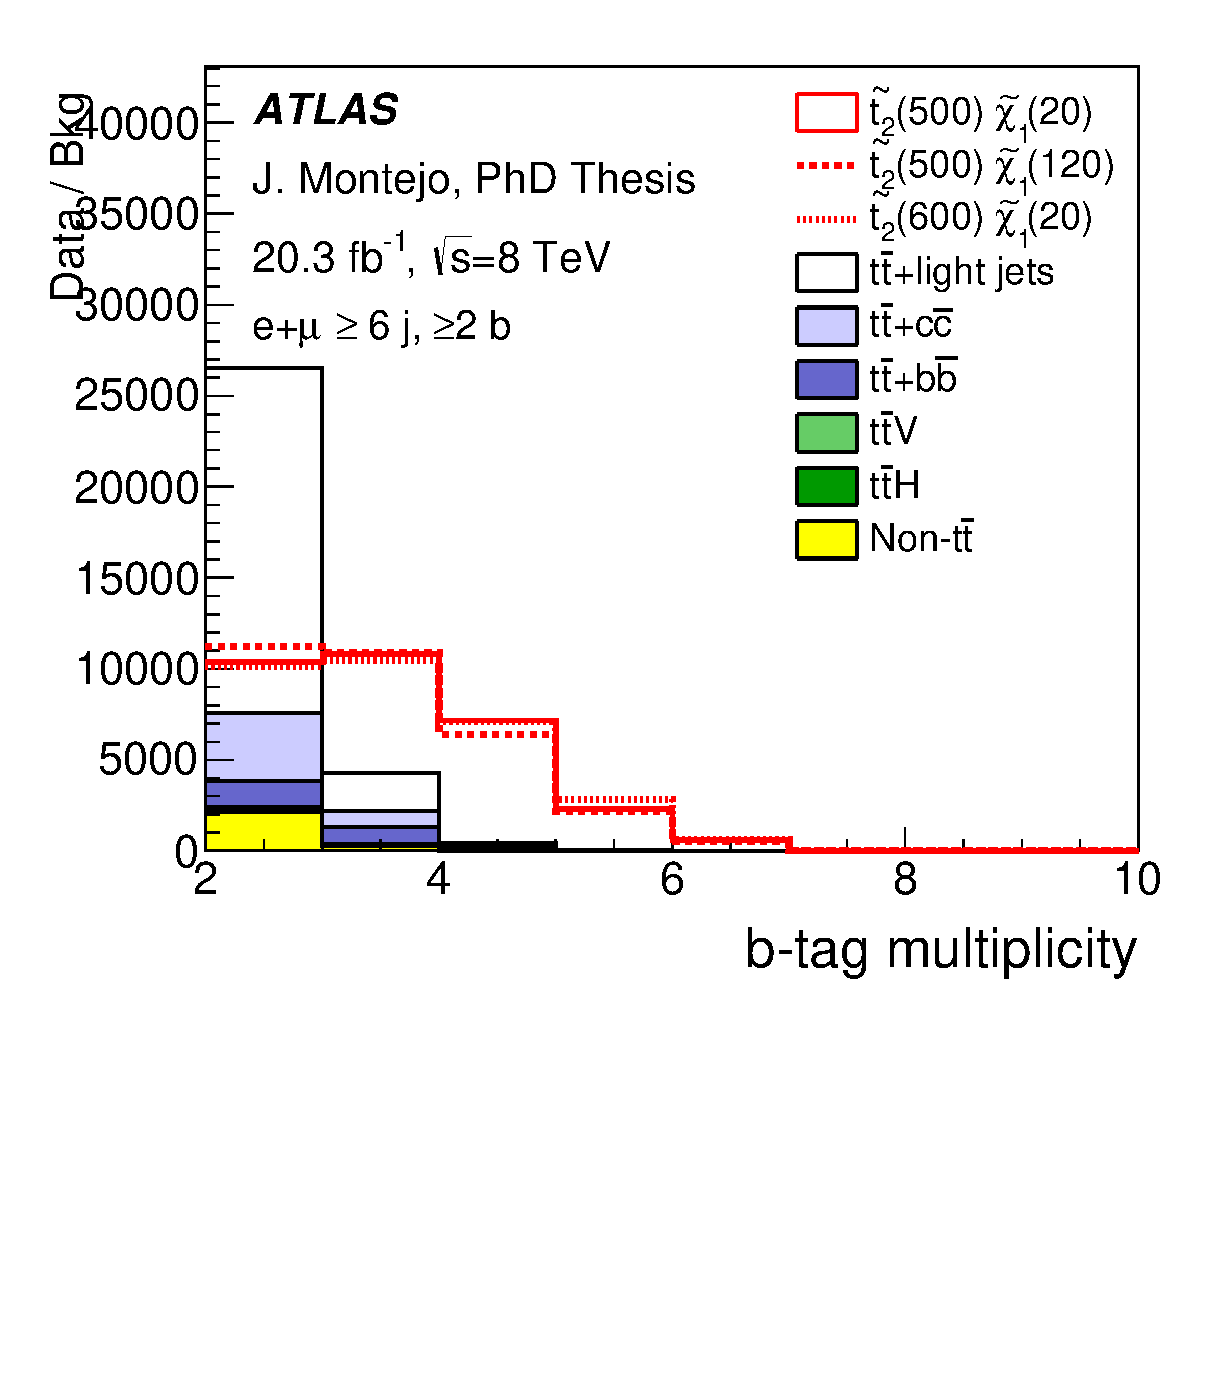
\includegraphics[trim=0cm 5cm 0cm 0cm, clip=true, width=\textwidth]{Analysis/Figures_stop2/plots_stop2/ELEMUON/6jetin/2btagin/bjet_n_ELEMUON_6jetin2btagin_NOMINAL}}\caption{}\label{fig:shapestop_nbtag}
    \end{subfigure}
\caption{Comparison of (a) the jet multiplicity distribution after preselection, and (b) the $b$-tag multiplicity distribution 
after the requirement of $\geq$6 jets, between the total background (shaded histogram) and several mass hypotheses for the signal.
}
\label{fig:shapestop_njet_nbtag}
\end{figure}

A large value of the \met\ is expected from the two neutralinos in the final state and the neutrino from the leptonic $W$ decay.
Figure~\ref{fig:shapestop_met} compares the \met\ distribution between signal and background for preselected events with $\geq 6$ jets in different $b$-tag regions.

\begin{figure}[!tp]
\centering
\begin{subfigure}{0.32\textwidth}
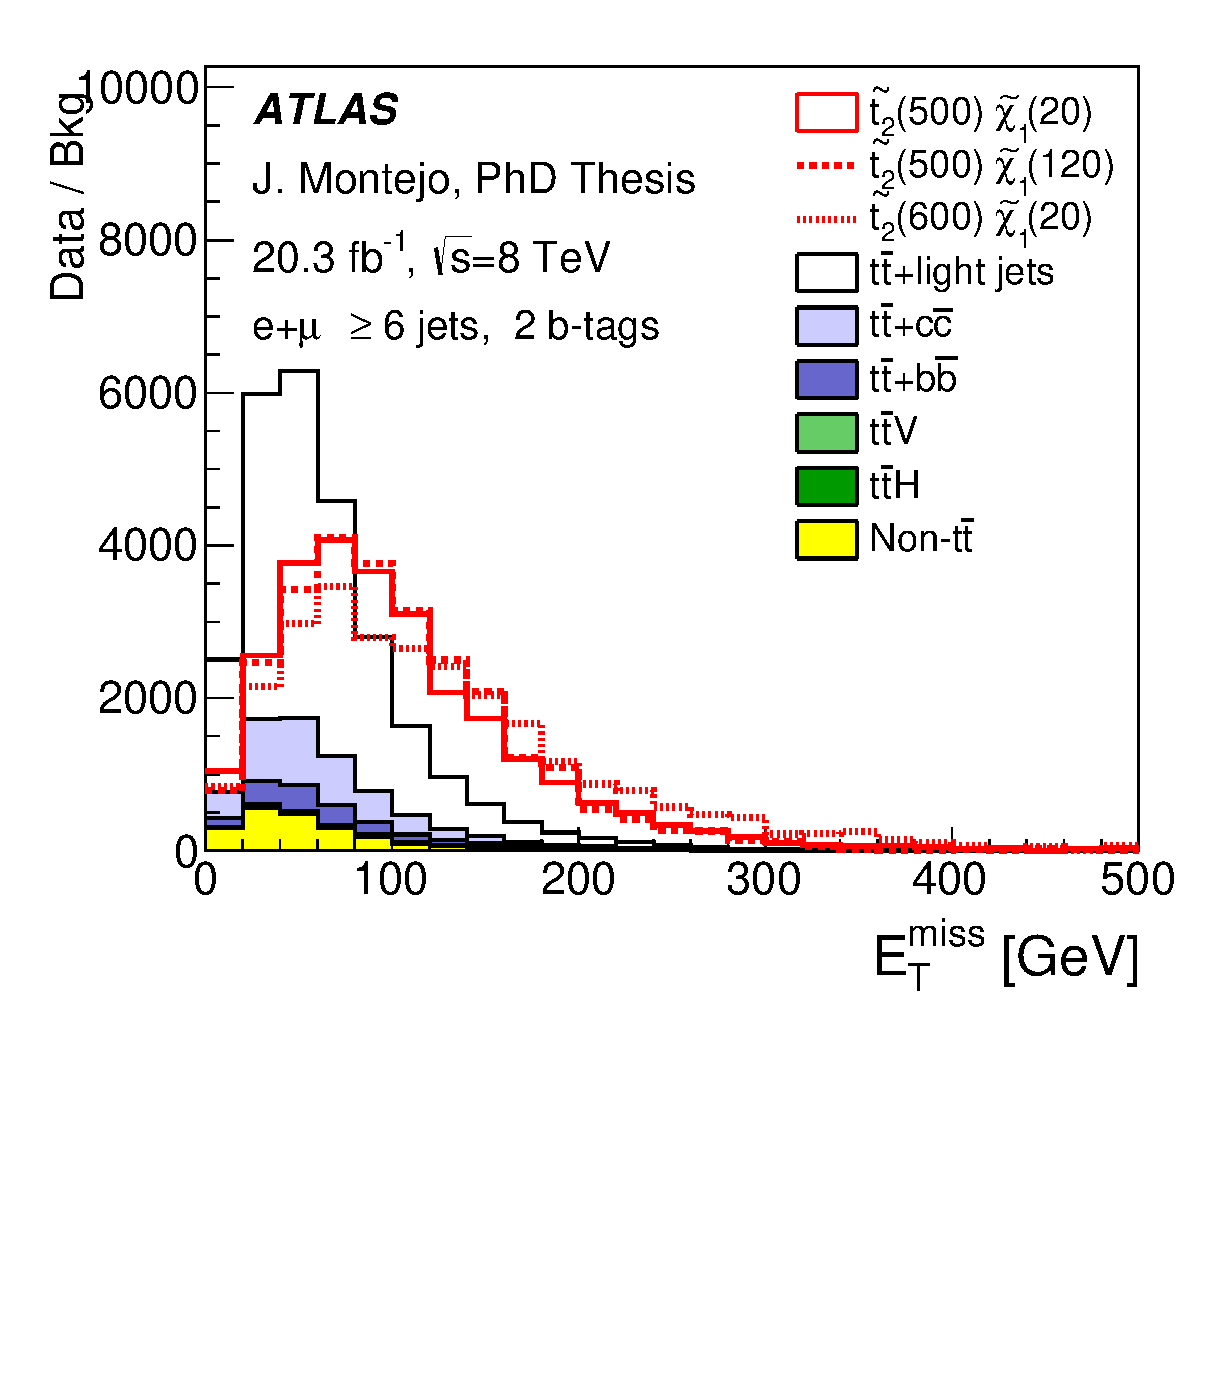
\includegraphics[trim=0cm 5cm 0cm 0cm, clip=true, width=\textwidth]{Analysis/Figures_stop2/plots_stop2/ELEMUON/6jetin/2btagex/met_ELEMUON_6jetin2btagex_NOMINAL}
\caption{}\end{subfigure}
\begin{subfigure}{0.32\textwidth}
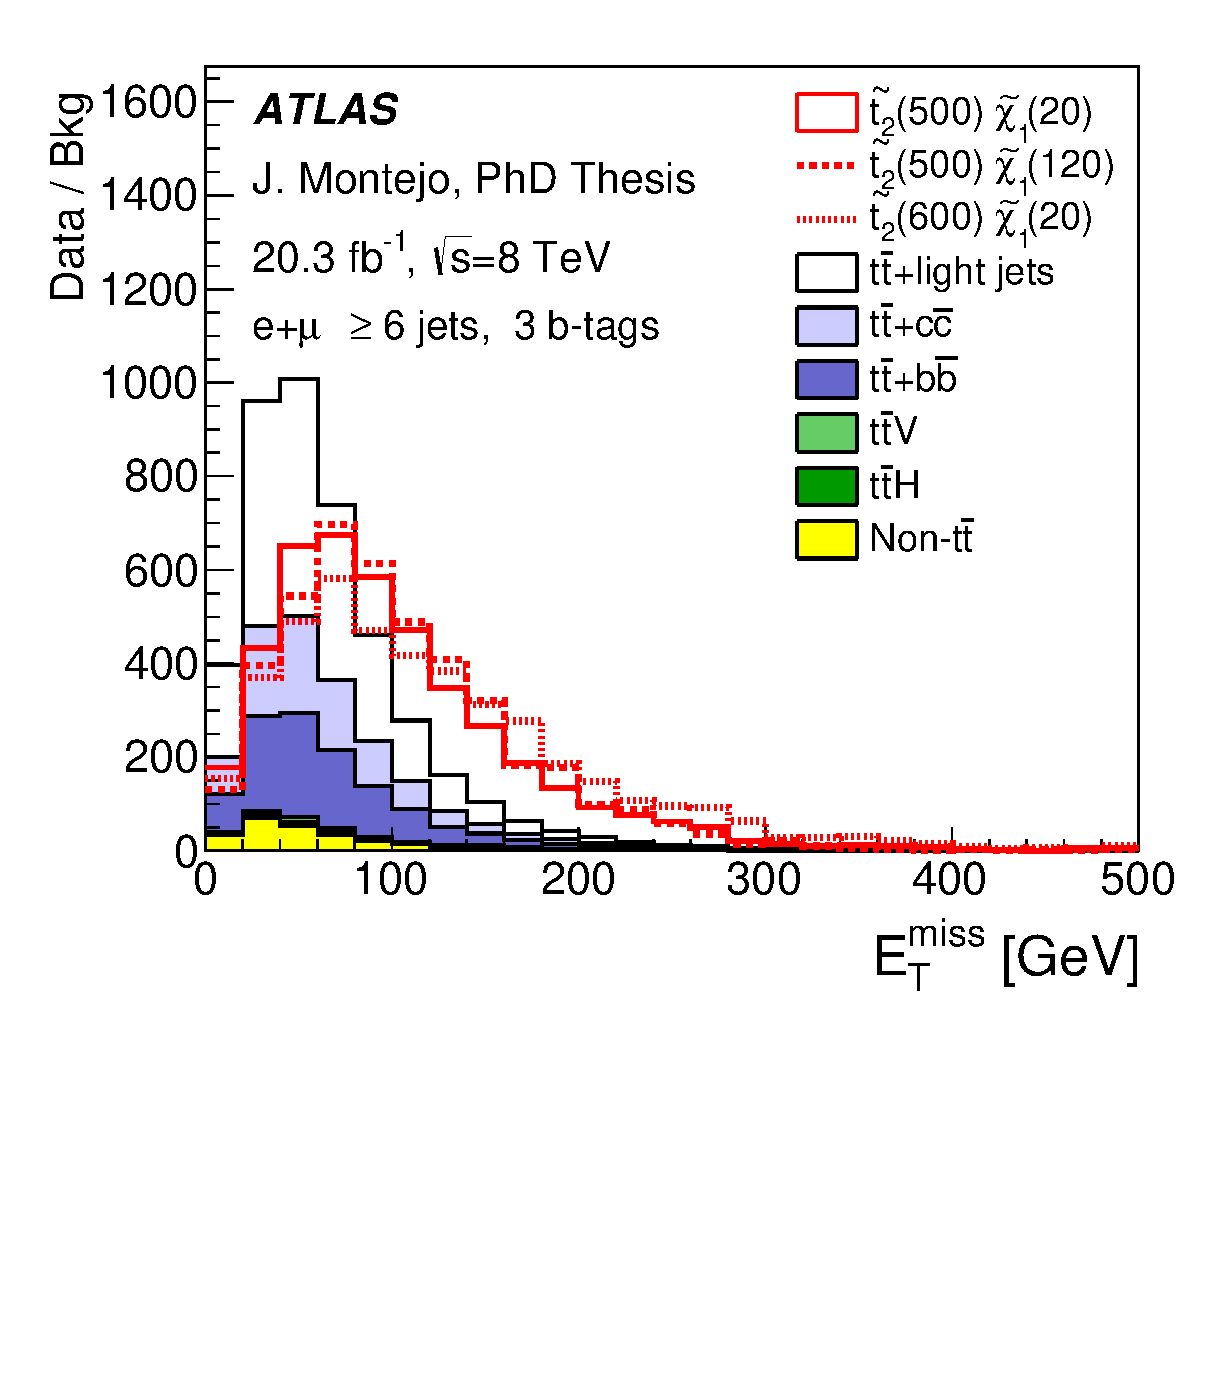
\includegraphics[trim=0cm 5cm 0cm 0cm, clip=true, width=\textwidth]{Analysis/Figures_stop2/plots_stop2/ELEMUON/6jetin/3btagex/met_ELEMUON_6jetin3btagex_NOMINAL}
\caption{}\end{subfigure}
\begin{subfigure}{0.32\textwidth}
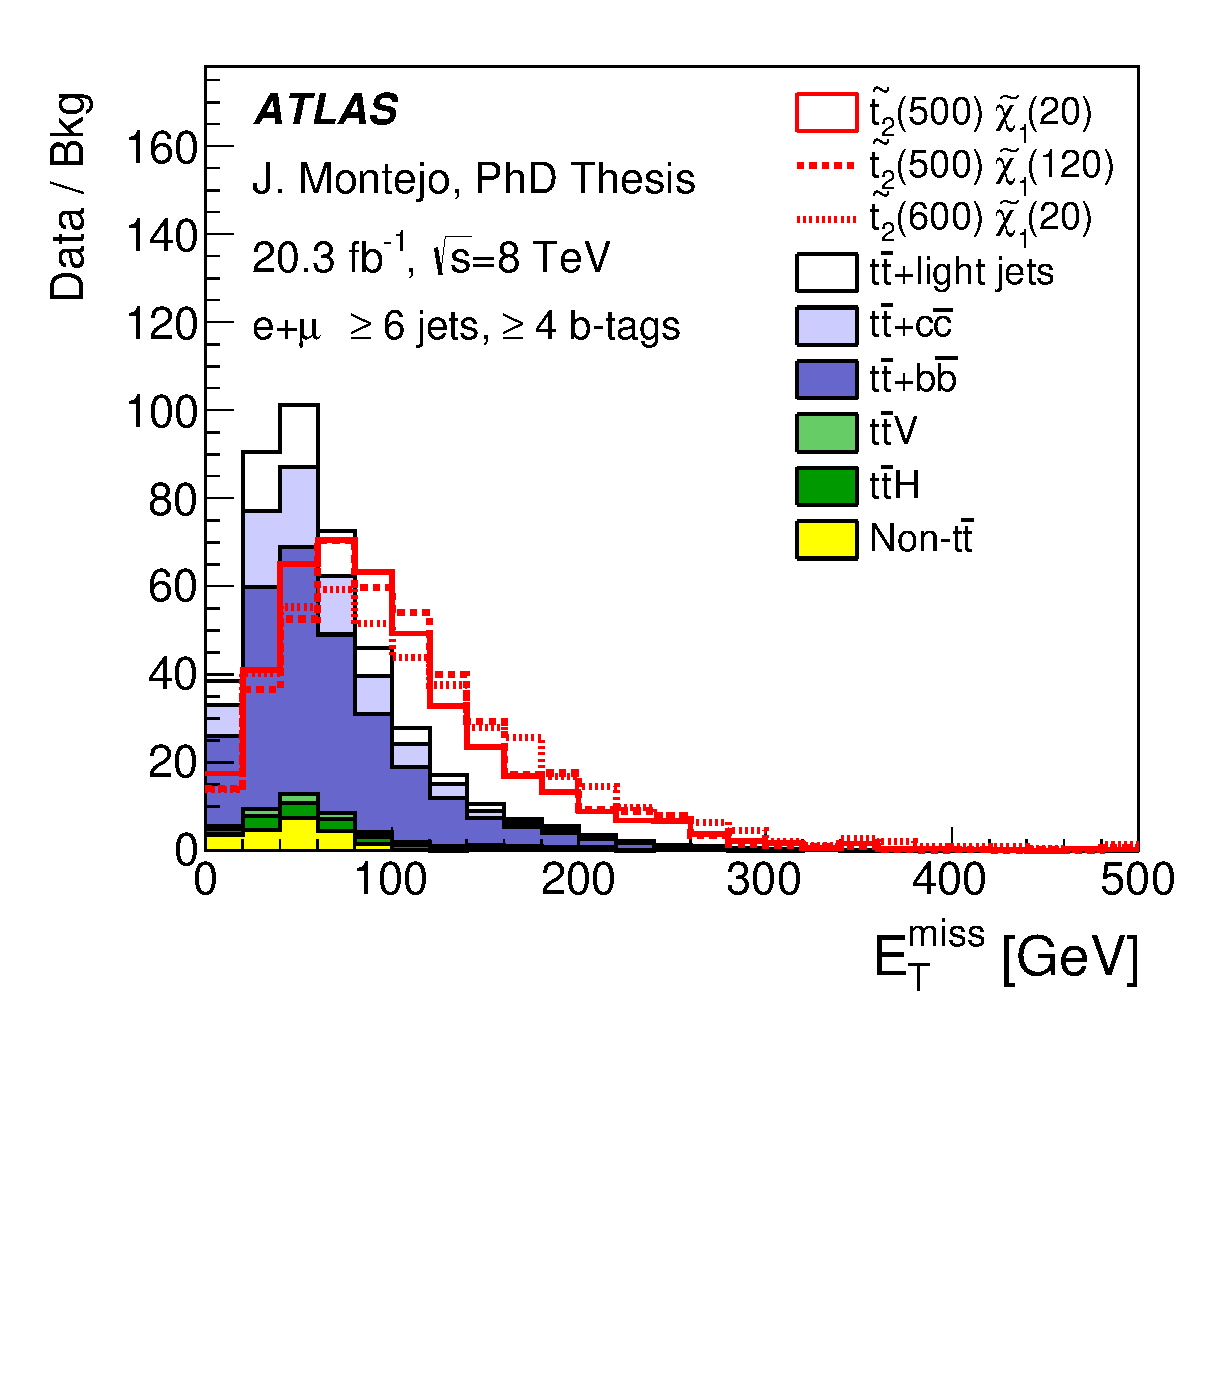
\includegraphics[trim=0cm 5cm 0cm 0cm, clip=true, width=\textwidth]{Analysis/Figures_stop2/plots_stop2/ELEMUON/6jetin/4btagin/met_ELEMUON_6jetin4btagin_NOMINAL}
\caption{}\end{subfigure}
\caption{Comparison of the distribution of \met\ in events with $\geq 6$ jets and (a) two $b$-tags, (b) three $b$-tags and (c) four or more $b$-tags.
  The signal is normalized to the background sum and three different mass hypotheses are shown.
}
\label{fig:shapestop_met}
\end{figure}

Following event selection cuts are introduced:
\begin{itemize}
  \item Given the high jet multiplicity, an additional requirement is introduced selecting events with $\geq$6 jets.
  \item A cut on the \met\ is introduced: $\met > \unit[50]{\gev}$.
\end{itemize}

The presence of \met\ is one of the common features of third-generation squarks analyses and is heavily exploited. However, \met\ has reduced discrimination power in this analysis due to two features: the presence of a neutrino in the main background, and the decay chain of the signal through multiple massive particles, thus reducing the available phase space for the boost of the neutralinos.
The difference in the origin of \met\ can further be exploited through the transverse mass of the leptonic $W$, \mtw.
Figure~\ref{fig:shapestop_WlepMT} compares the \mtw\ distribution between signal and background after the analysis cuts are applied, for the different $b$-tag regions.
The background peaks below $m_W \sim \unit[80]{\gev}$ as expected, and falls rapidly for high \mtw. The signal distribution has no clear peak and tends towards higher values of \mtw. Since no clear cut can be placed without losing a large fraction of the signal, regions are split into two subchannels depending on the value of \mtw.

The selected events are categorized in different channels depending on the number of $b$-tagged jets (2, 3 and $\geq 4$), 
and on the value of \mtw: $\mtw < \unit[120]{\gev}$ (``low \mtw'') and $\mtw \geq \unit[120]{\gev}$ (``high \mtw'').
Therefore a total of six analysis channels are considered, where the most sensitive one is ($\geq 4$ $b$-tags, $\mtw \geq \unit[120]{\gev}$).

\begin{figure}[!tp]
\centering
\begin{subfigure}{0.32\textwidth}
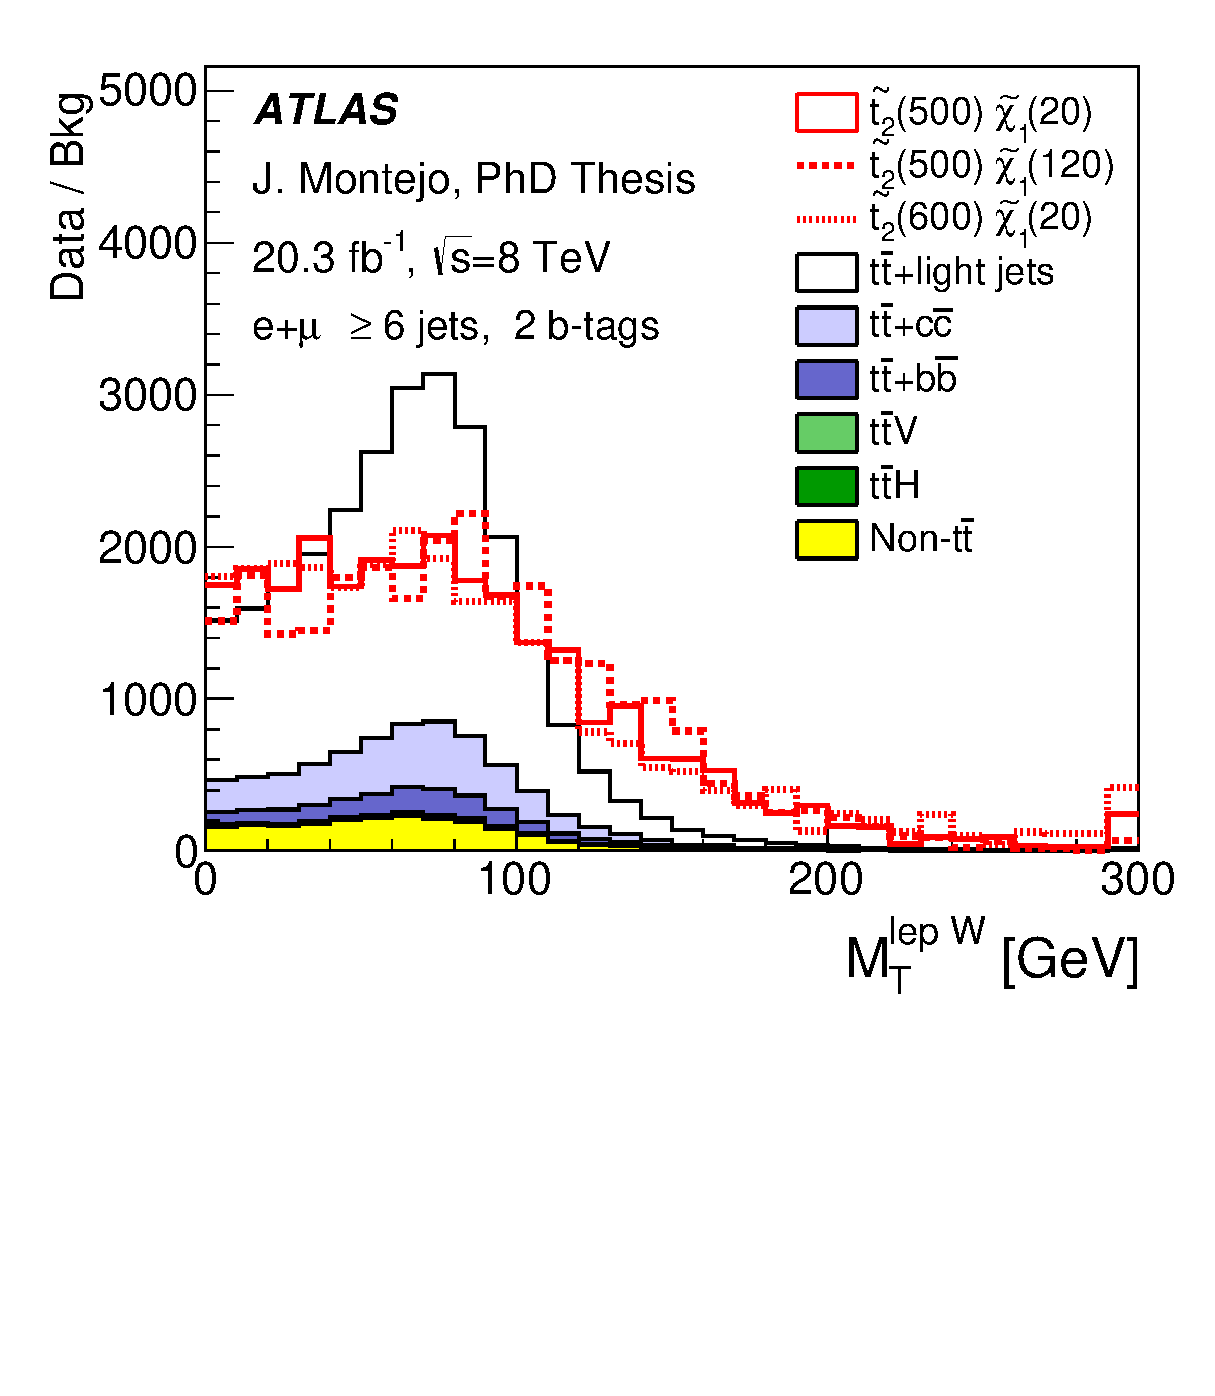
\includegraphics[trim=0cm 5cm 0cm 0cm, clip=true, width=\textwidth]{Analysis/Figures_stop2/plots_stop2/ELEMUON/6jetin/2btagex/WlepMT_ELEMUON_6jetin2btagex_NOMINAL}
\caption{}\end{subfigure}
\begin{subfigure}{0.32\textwidth}
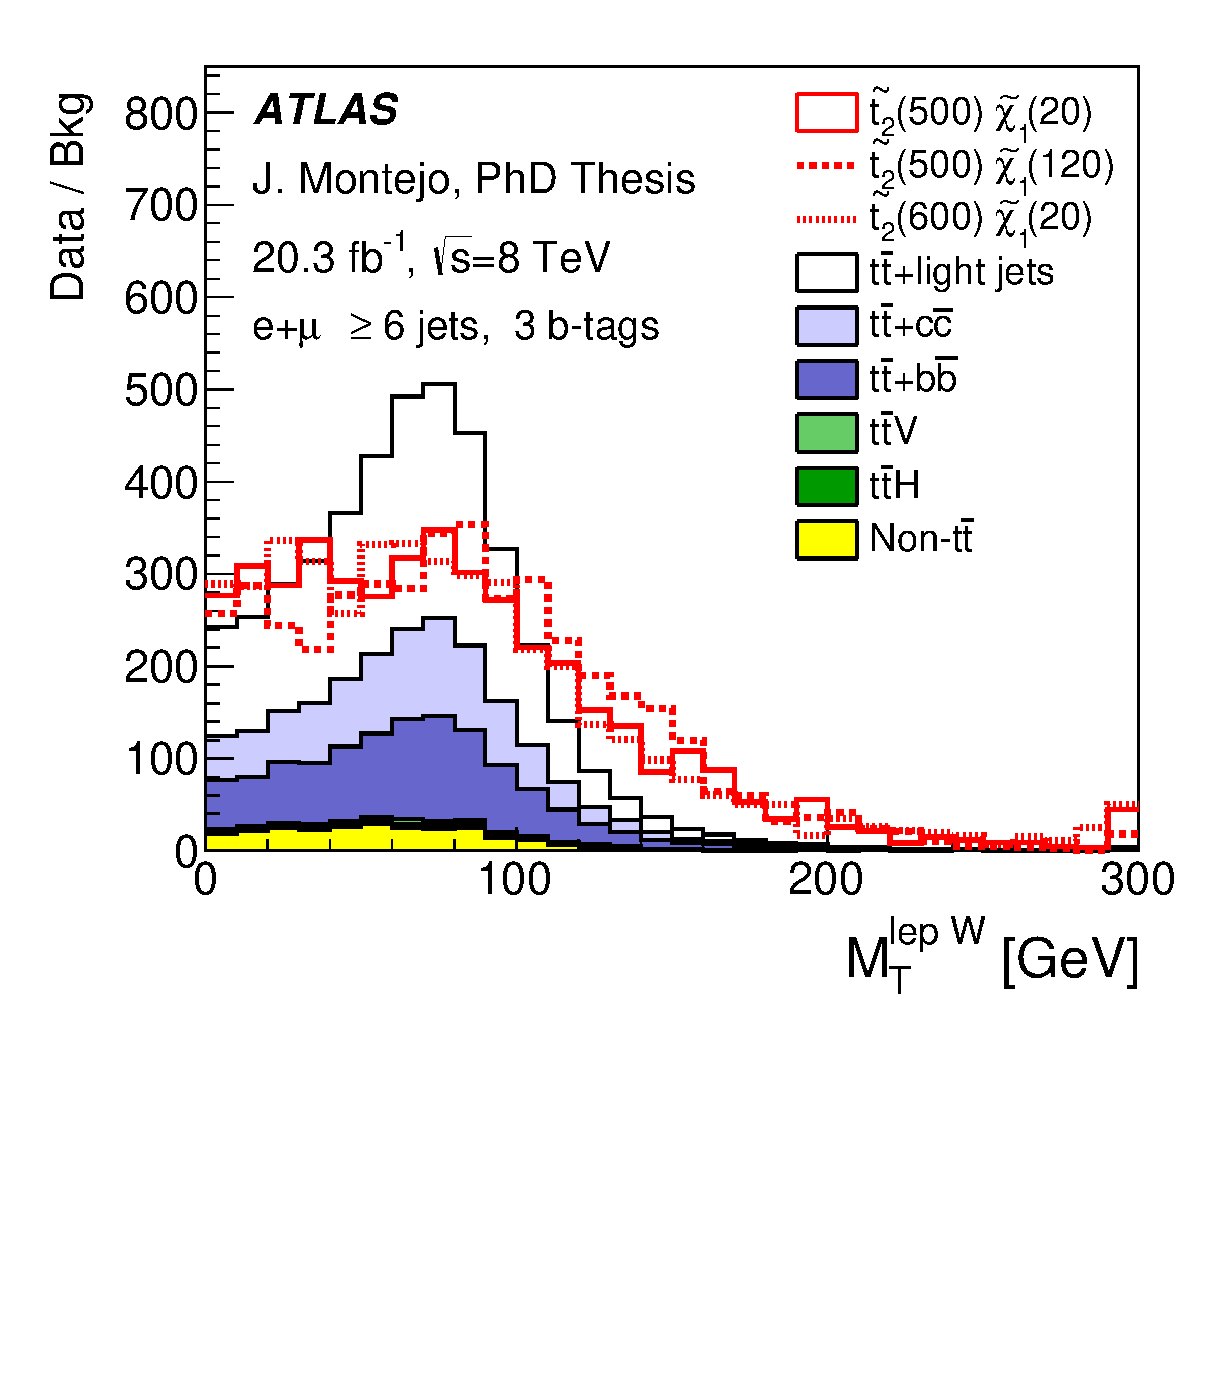
\includegraphics[trim=0cm 5cm 0cm 0cm, clip=true, width=\textwidth]{Analysis/Figures_stop2/plots_stop2/ELEMUON/6jetin/3btagex/WlepMT_ELEMUON_6jetin3btagex_NOMINAL}
\caption{}\end{subfigure}
\begin{subfigure}{0.32\textwidth}
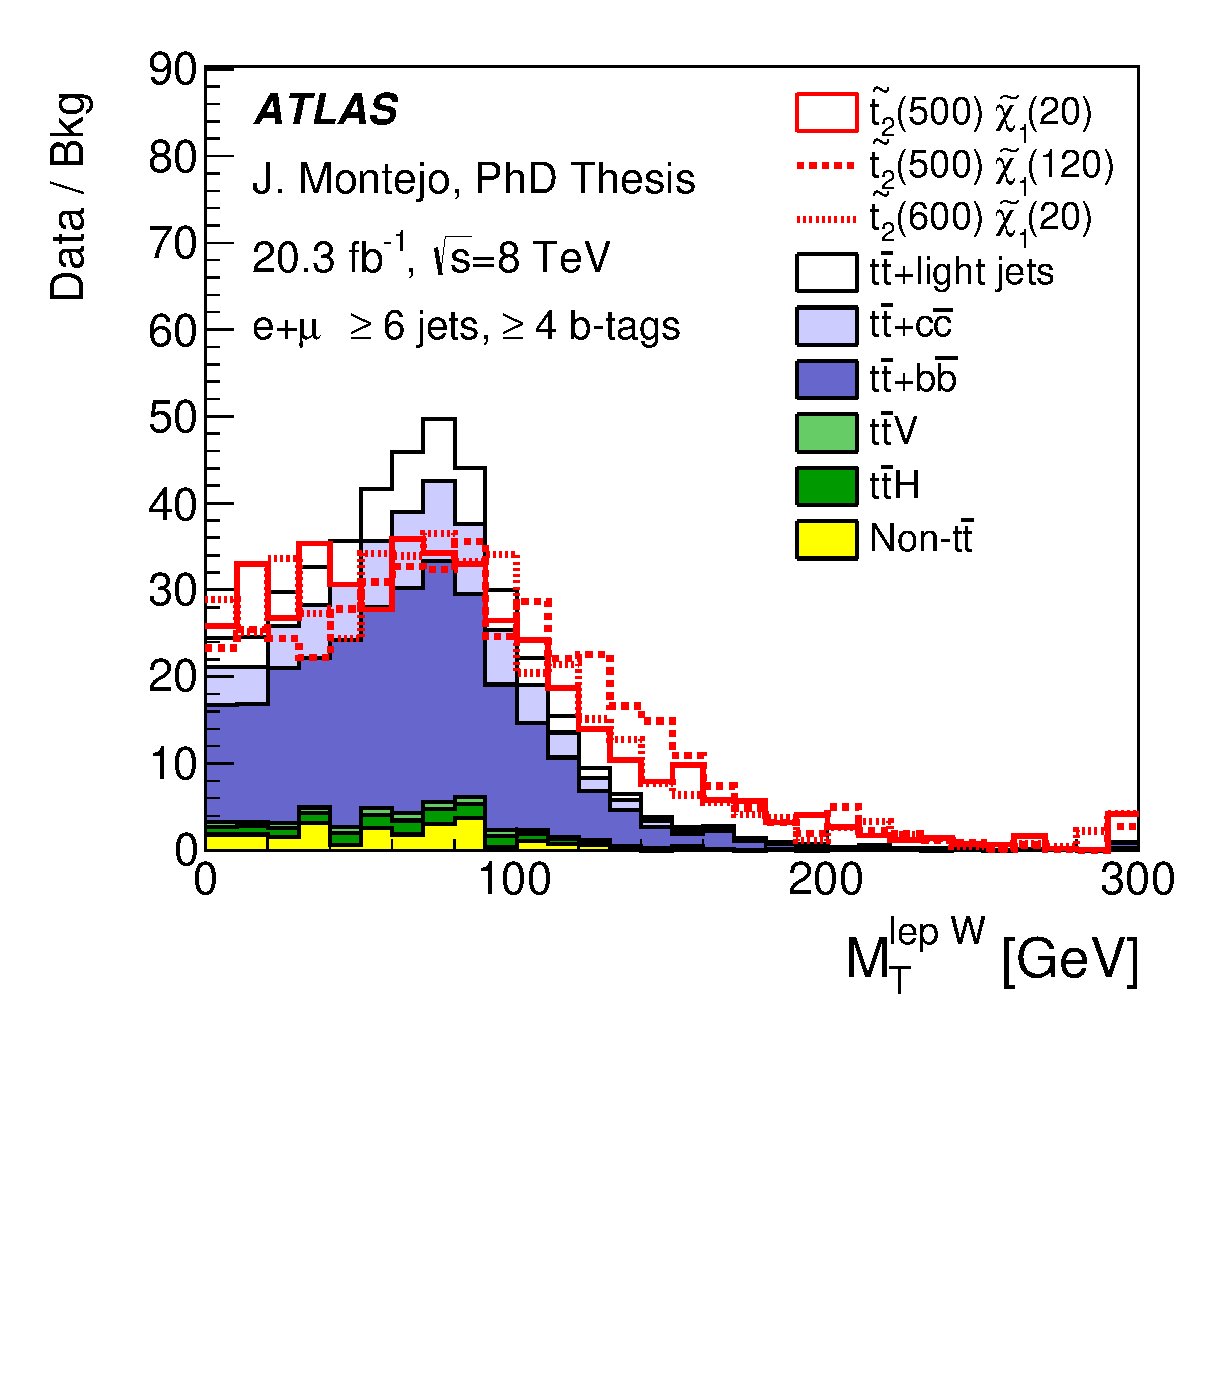
\includegraphics[trim=0cm 5cm 0cm 0cm, clip=true, width=\textwidth]{Analysis/Figures_stop2/plots_stop2/ELEMUON/6jetin/4btagin/WlepMT_ELEMUON_6jetin4btagin_NOMINAL}
\caption{}\end{subfigure}
\caption{Comparison of the distribution of \mtw\ in events with $\geq 6$ jets and (a) two $b$-tags, (b) three $b$-tags and (c) four or more $b$-tags.
  The signal is normalized to the background sum and three different mass hypotheses are shown.
}
\label{fig:shapestop_WlepMT}
\end{figure}

\subsection{Discriminant variable: $\htnol$}

To further improve the separation between signal and background, the distinct kinematic features of the signal are exploited.
As already discussed, the signal is characterized by a higher average $\met$ and jet multiplicity than the background.
The latter results in a higher scalar sum of the jet $\pt$, referred to as $\hthad$.
In contrast, the lepton $\pt$ distribution, resulting from the $W$ boson decay, is often similar, or even softer than that of the background.
This is demonstrated in figure~\ref{fig:kinematics}. Therefore, instead of considering the traditional scalar sum of the lepton $\pt$, $\met$
and jet $\pt$ (i.e. $\HT$) as the discriminating variable between signal and background, this analysis considers only
the $\met$ and jets in such sum, referred to as: $\htnol = \met + \hthad$.

\begin{figure}[!tp]
\centering
\begin{subfigure}{0.32\textwidth}
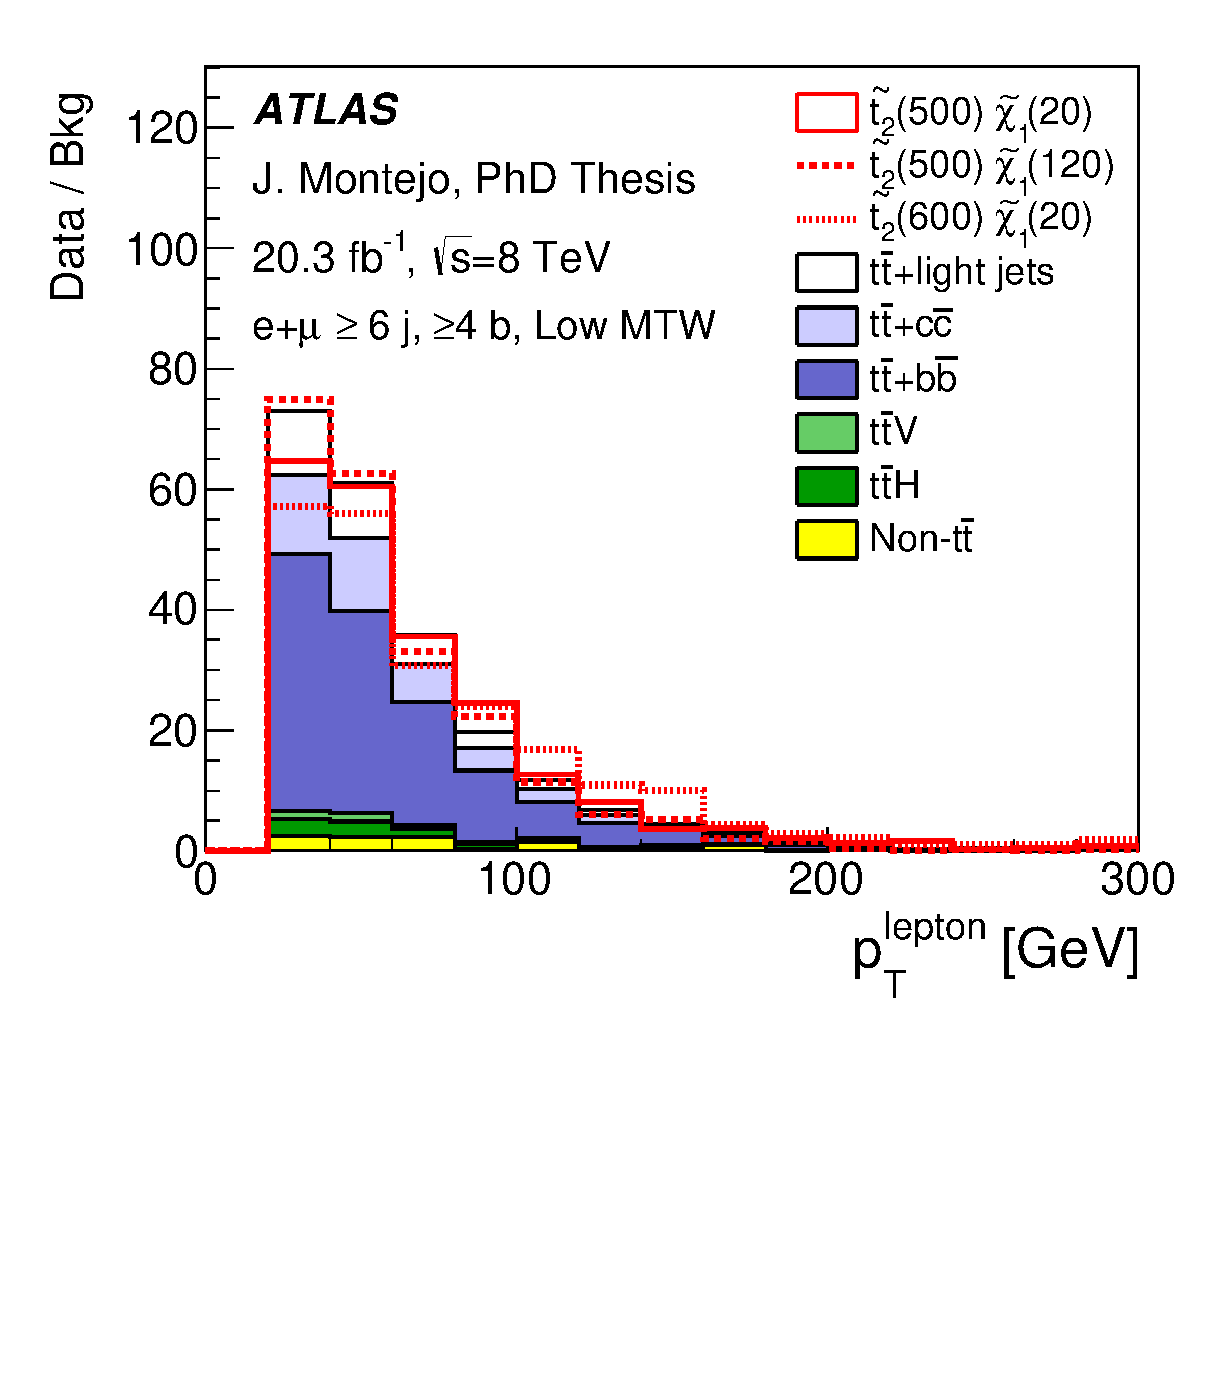
\includegraphics[trim=0cm 5cm 0cm 0cm, clip=true, width=\textwidth]{Analysis/Figures_stop2/plots_stop2_lowMTW/ELEMUON/6jetin/4btagin/lep_pt_ELEMUON_6jetin4btagin_NOMINAL}
\caption{}\end{subfigure}
\begin{subfigure}{0.32\textwidth}
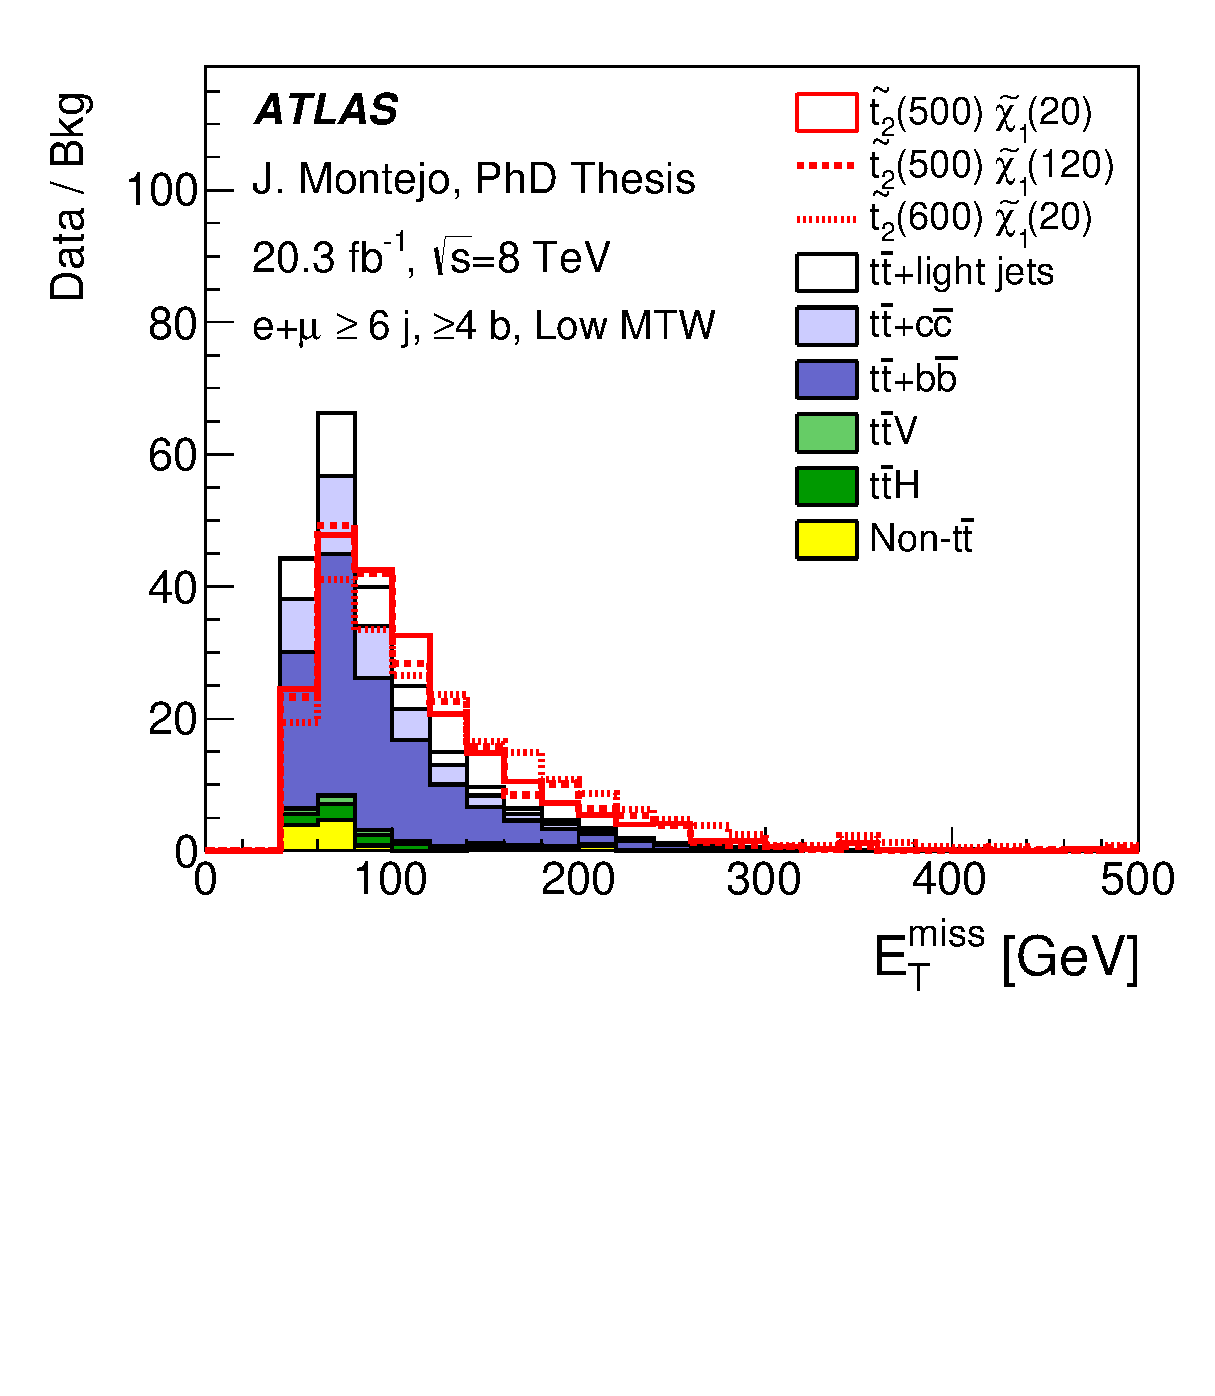
\includegraphics[trim=0cm 5cm 0cm 0cm, clip=true, width=\textwidth]{Analysis/Figures_stop2/plots_stop2_lowMTW/ELEMUON/6jetin/4btagin/met_ELEMUON_6jetin4btagin_NOMINAL}
\caption{}\end{subfigure}
\begin{subfigure}{0.32\textwidth}
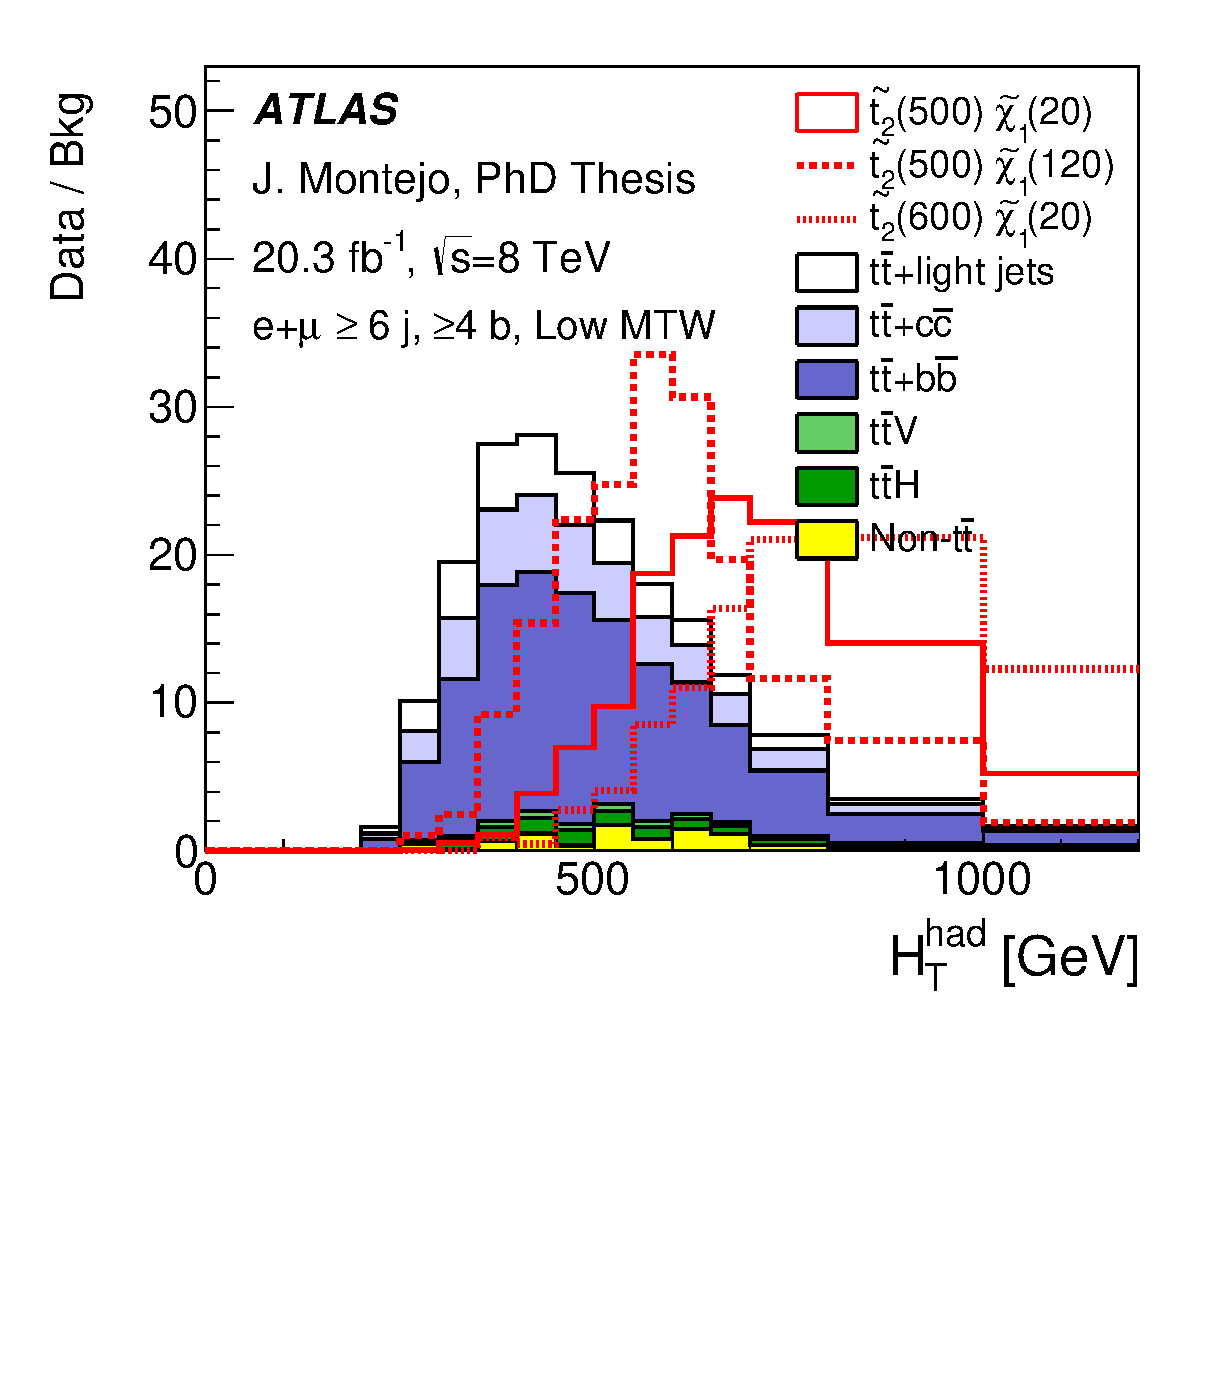
\includegraphics[trim=0cm 5cm 0cm 0cm, clip=true, width=\textwidth]{Analysis/Figures_stop2/plots_stop2_lowMTW/ELEMUON/6jetin/4btagin/HTj_ELEMUON_6jetin4btagin_NOMINAL} \\
\caption{}\end{subfigure}
\begin{subfigure}{0.32\textwidth}
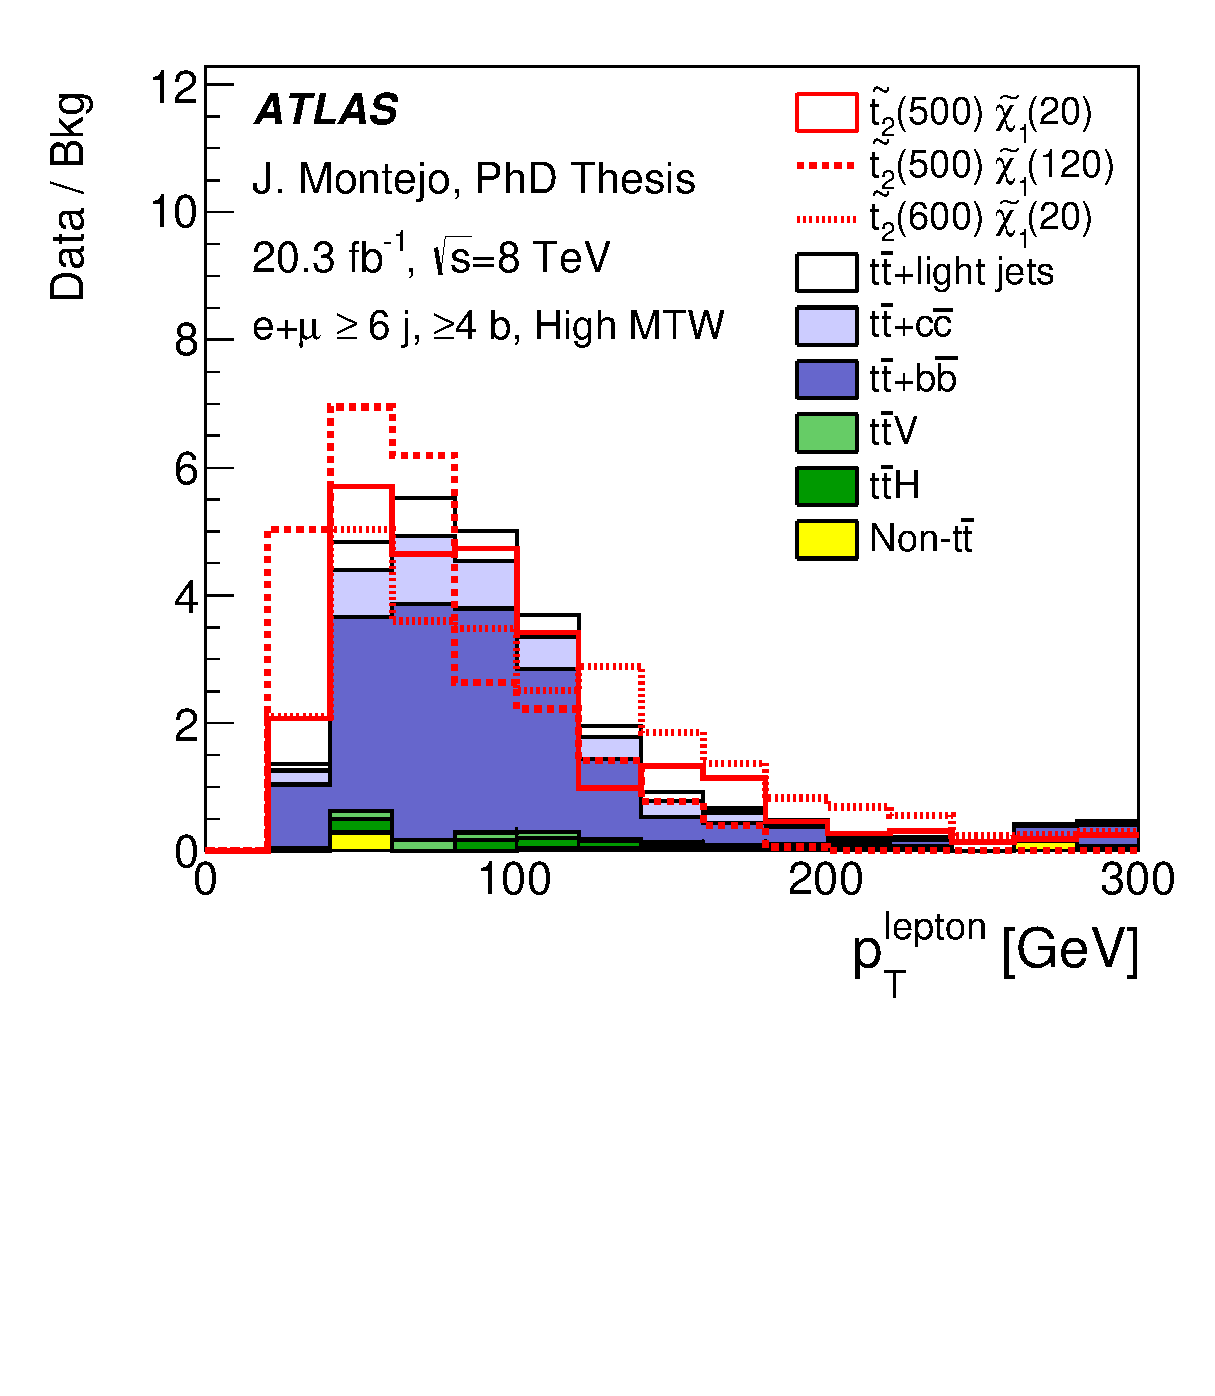
\includegraphics[trim=0cm 5cm 0cm 0cm, clip=true, width=\textwidth]{Analysis/Figures_stop2/plots_stop2_highMTW/ELEMUON/6jetin/4btagin/lep_pt_ELEMUON_6jetin4btagin_NOMINAL}
\caption{}\end{subfigure}
\begin{subfigure}{0.32\textwidth}
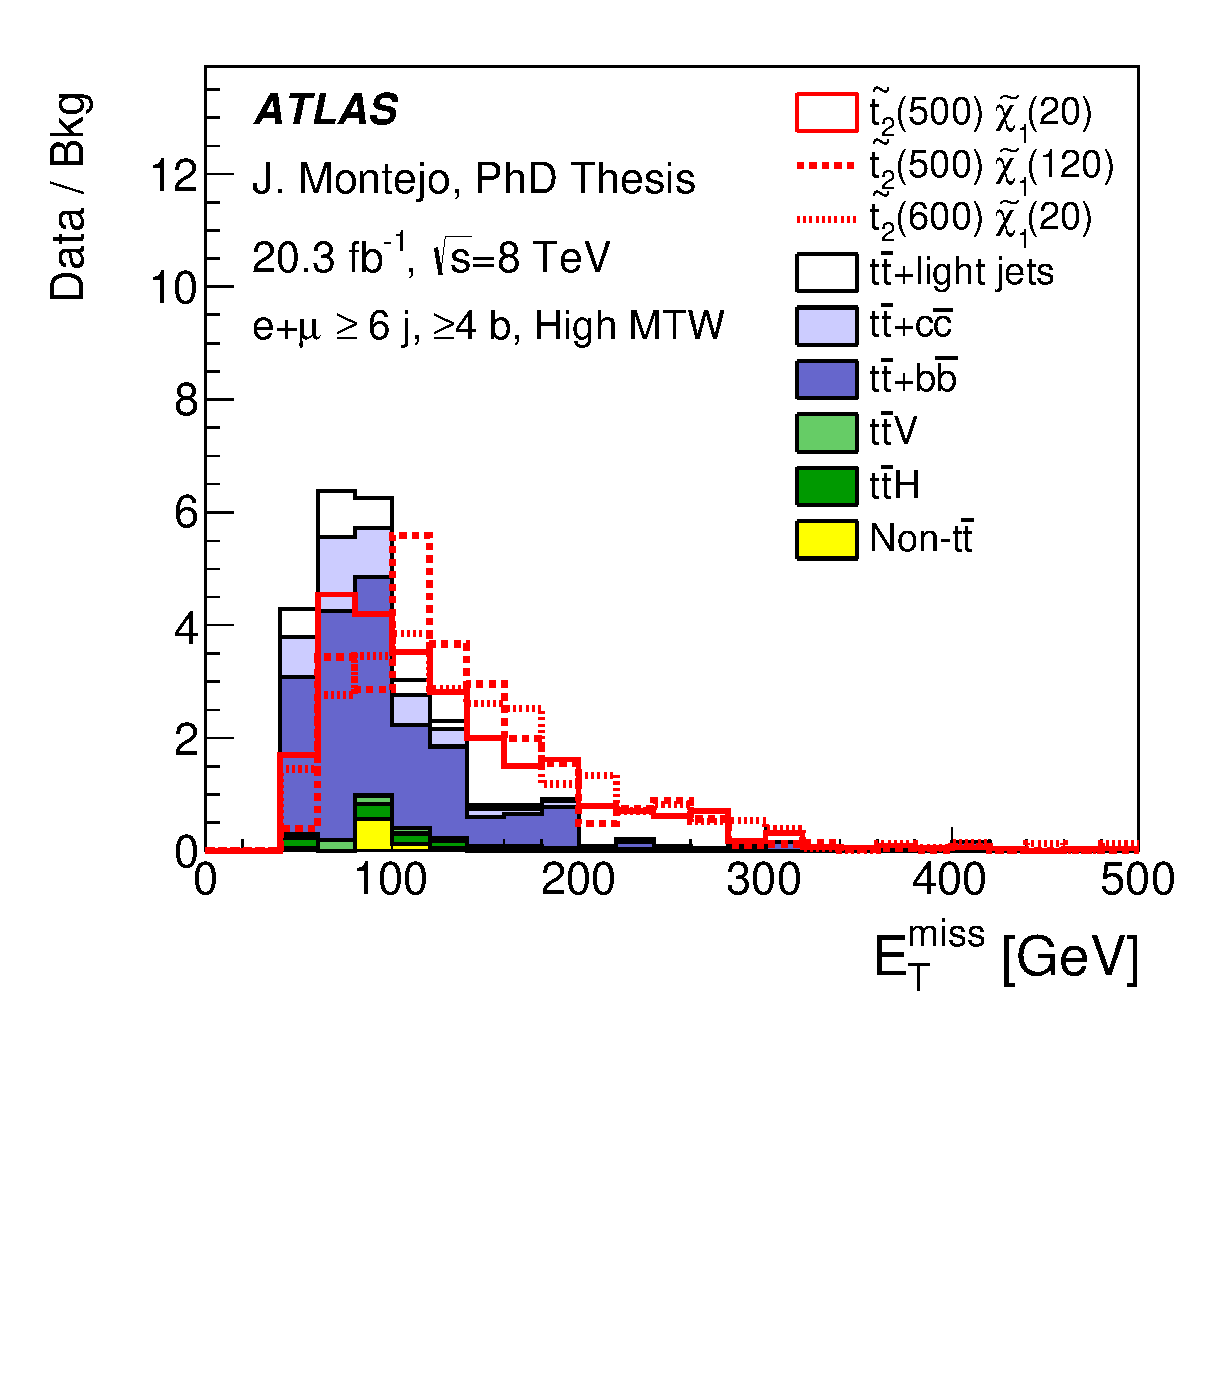
\includegraphics[trim=0cm 5cm 0cm 0cm, clip=true, width=\textwidth]{Analysis/Figures_stop2/plots_stop2_highMTW/ELEMUON/6jetin/4btagin/met_ELEMUON_6jetin4btagin_NOMINAL}
\caption{}\end{subfigure}
\begin{subfigure}{0.32\textwidth}
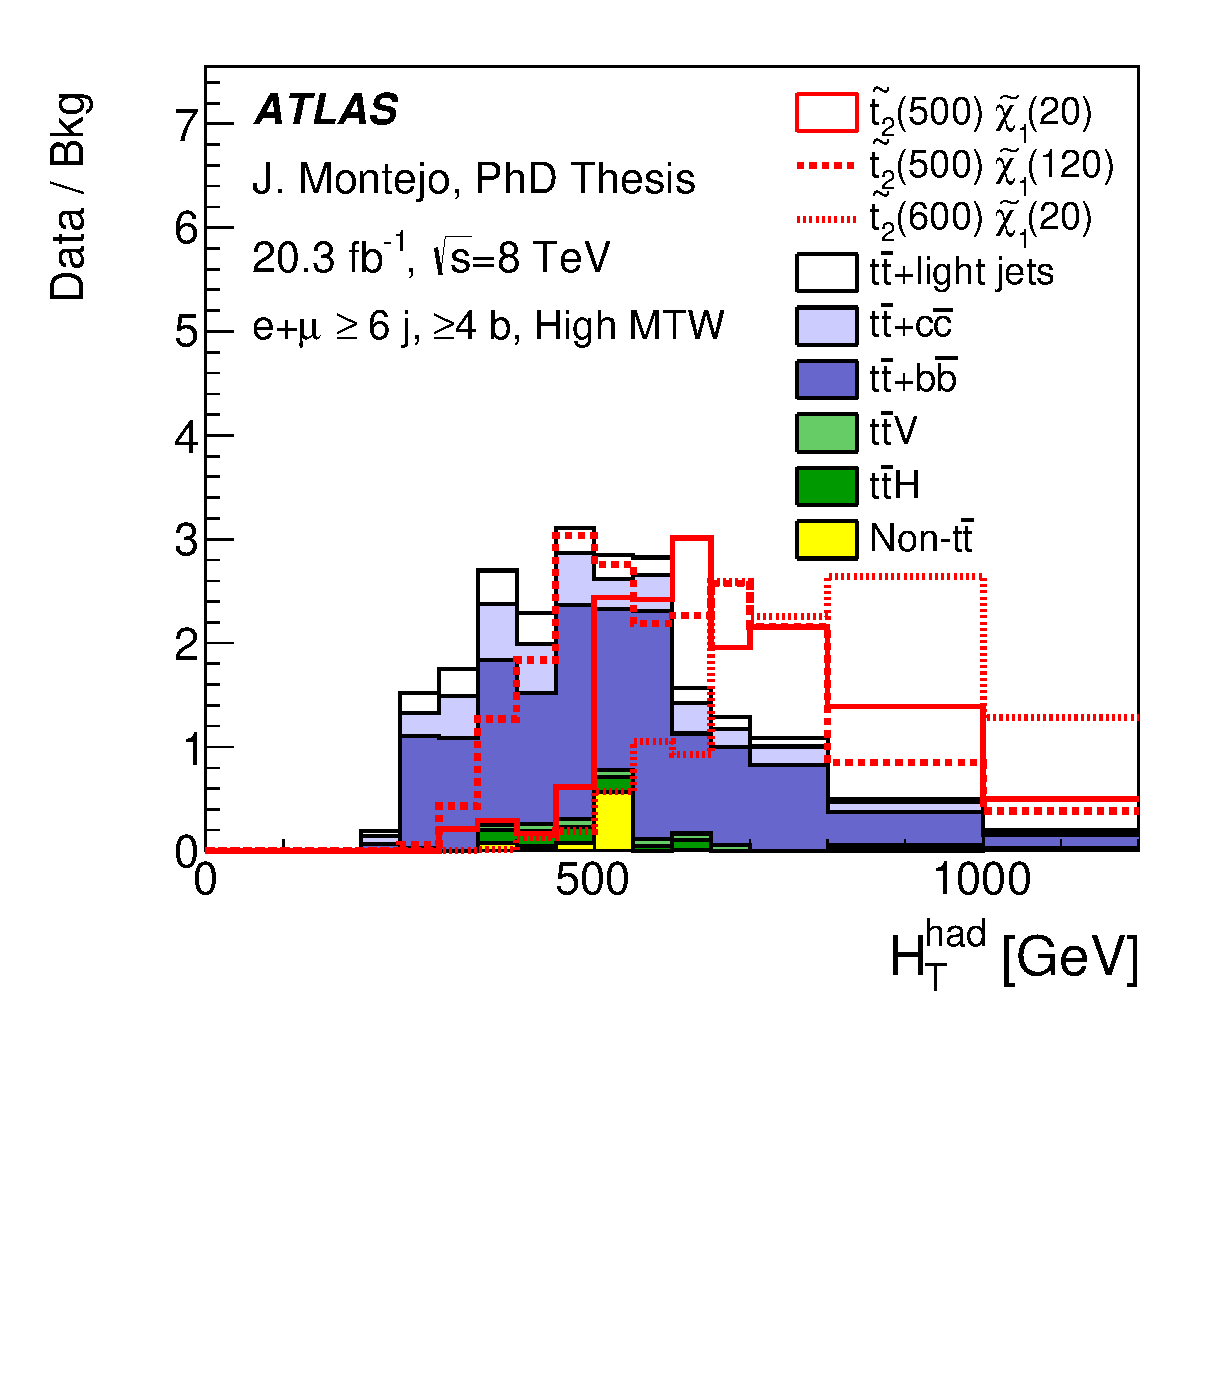
\includegraphics[trim=0cm 5cm 0cm 0cm, clip=true, width=\textwidth]{Analysis/Figures_stop2/plots_stop2_highMTW/ELEMUON/6jetin/4btagin/HTj_ELEMUON_6jetin4btagin_NOMINAL} \\
\caption{}\end{subfigure}
\caption{Comparison of the distributions of lepton \pt\ (left), \met\ (middle) and $\hthad$ (right) in events with $\geq 6$ jets, $\geq 4$ $b$-tags and low \mtw\ (top) or high \mtw\ (bottom).
  The signal is normalized to the background sum and three different mass hypotheses are shown.
}
\label{fig:kinematics}
\end{figure}

Figure~\ref{fig:HTnolep_prefit} shows the comparison of data and prediction for the $\htnol$ distributions for the six analysis
channels considered. The corresponding predicted and observed yields per channel can be found in table~\ref{tab:Prefit_Yields_stop2}.
At low $b$-tag multiplicity the contribution from $\st_1\bar{\st}_1$
production is not completely negligible and the splitting of the analysis in ``low $\mtw$''  ``high $\mtw$'' channels
provides some sensitivity to it. Therefore the $\st_1\bar{\st}_1$ process is also treated as signal in the analysis. 

%%%%%%%%%%%%%%
\begin{figure}[tpb!]
\begin{center}
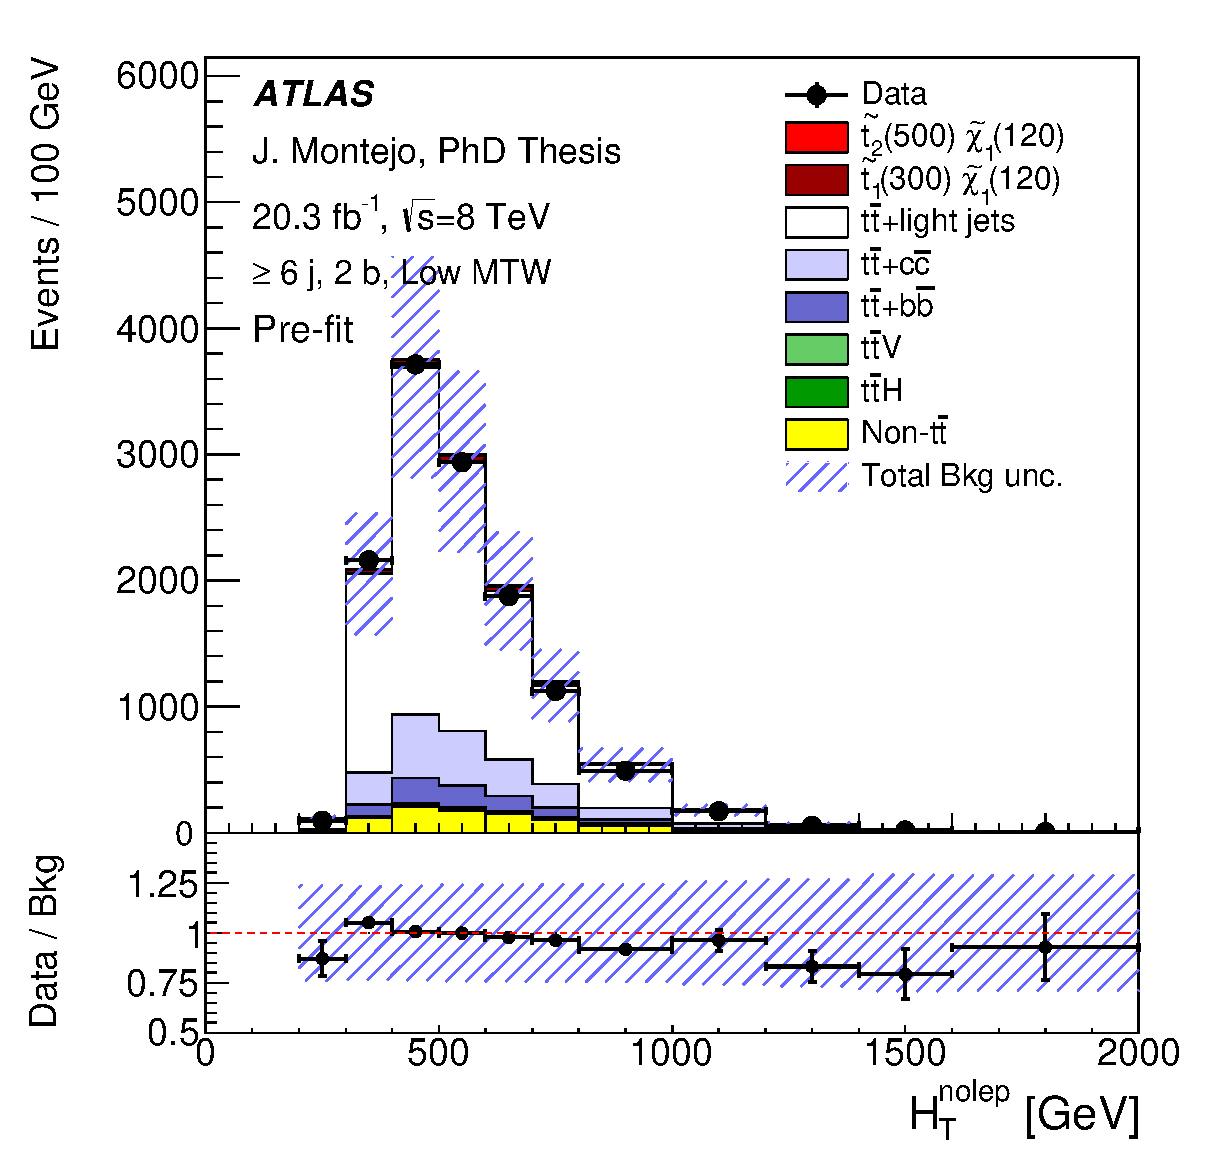
\includegraphics[width=0.41\textwidth]{Analysis/Figures_stop2/Prefit_HTnolep_unblind//HTnolep_6jetin2btagexLowMTW8TeV.eps} 
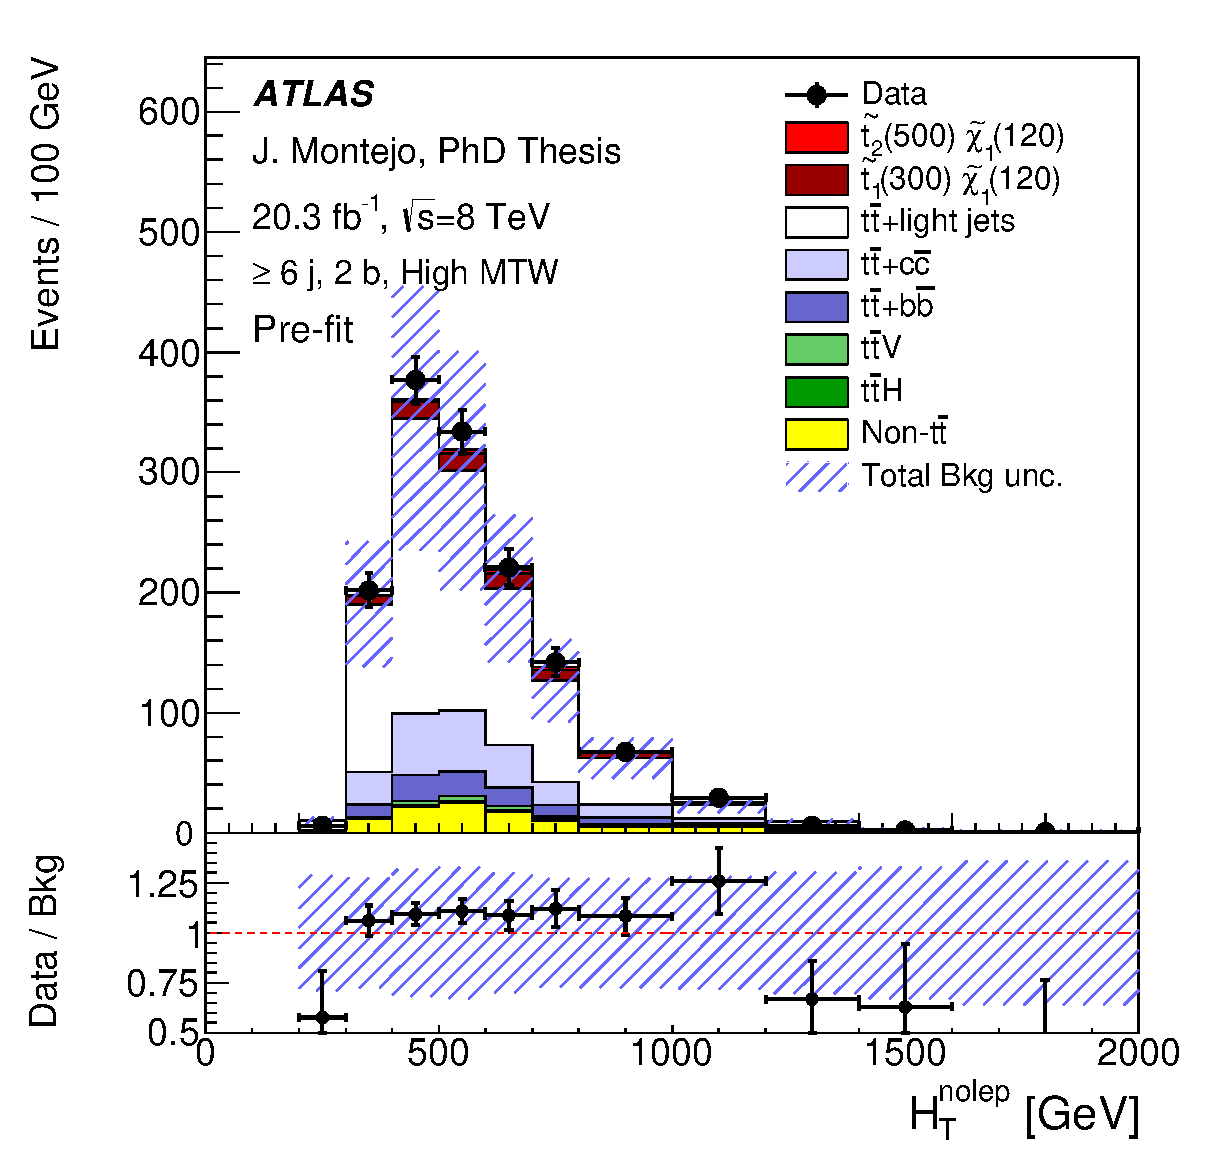
\includegraphics[width=0.41\textwidth]{Analysis/Figures_stop2/Prefit_HTnolep_unblind//HTnolep_6jetin2btagexHighMTW8TeV.eps} \\
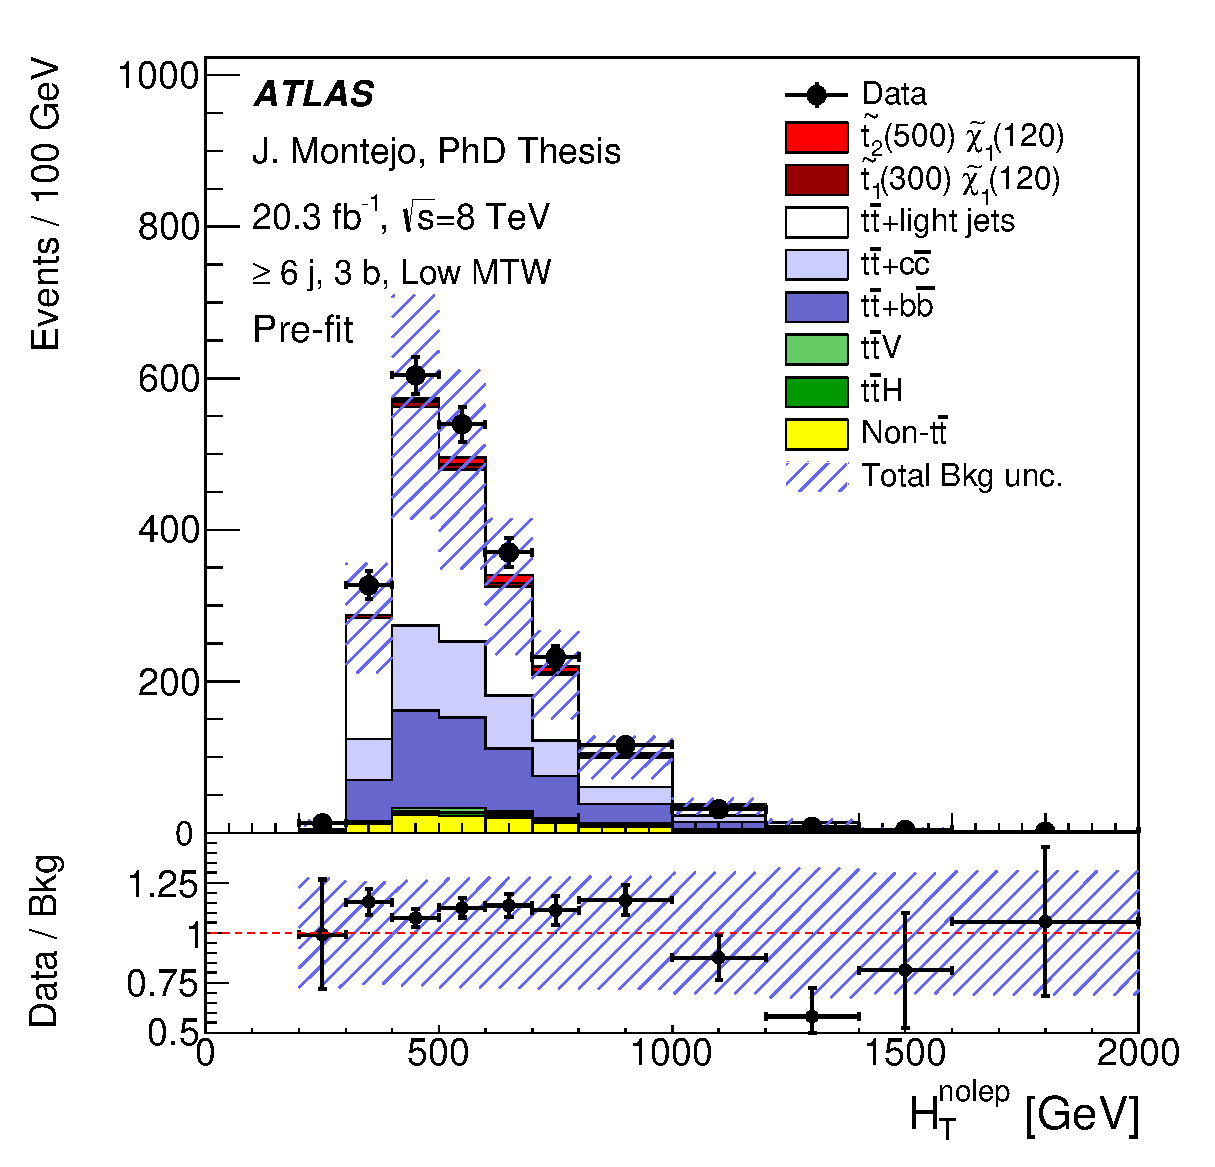
\includegraphics[width=0.41\textwidth]{Analysis/Figures_stop2/Prefit_HTnolep_unblind//HTnolep_6jetin3btagexLowMTW8TeV.eps}
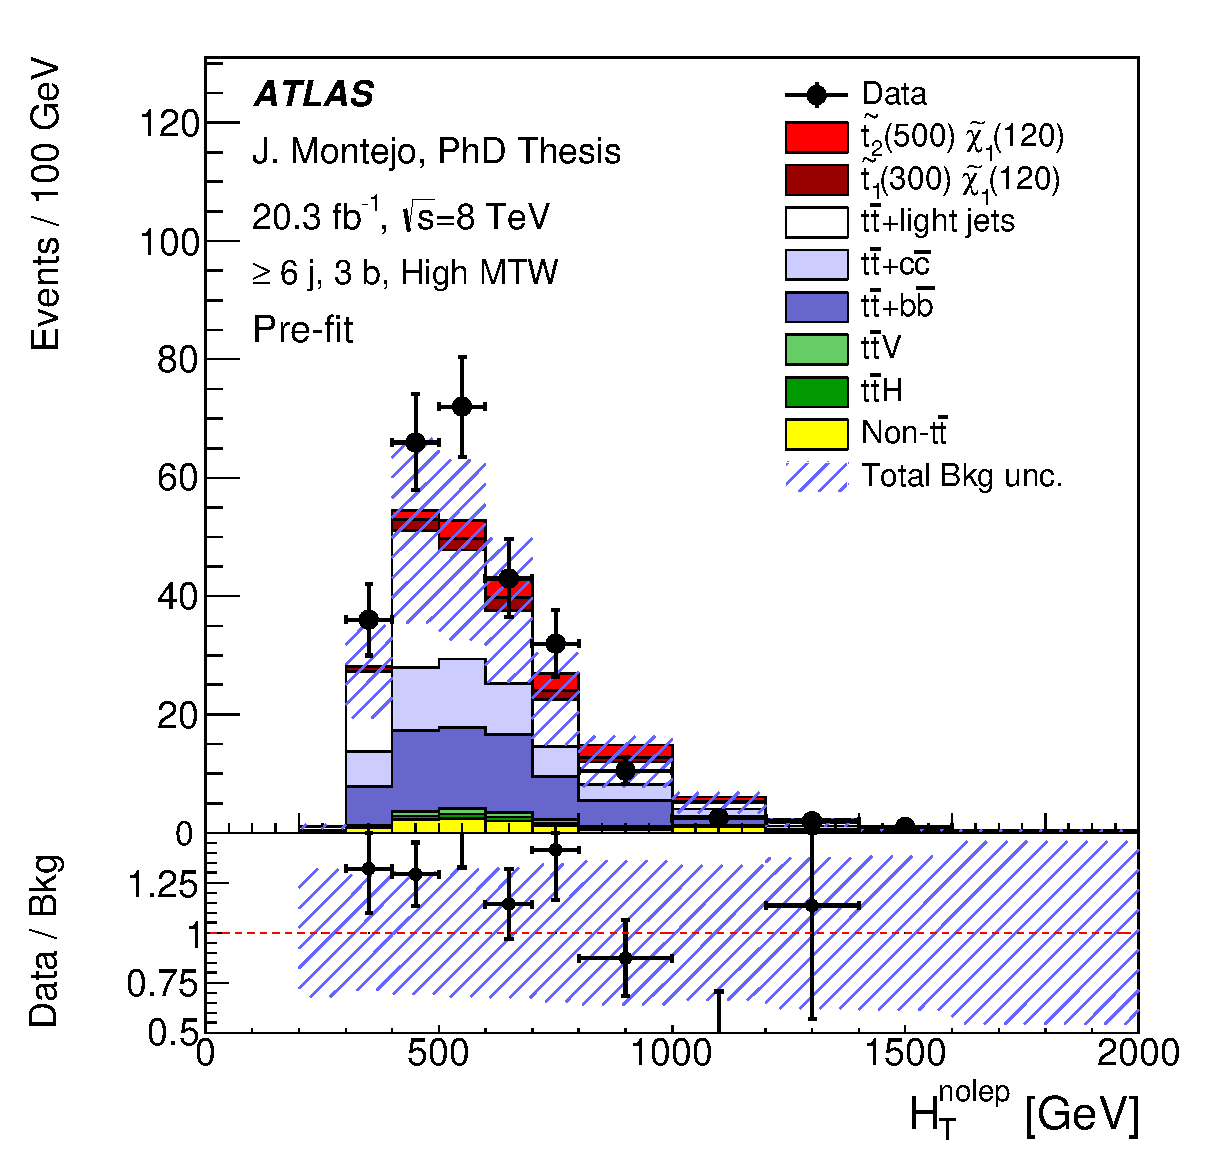
\includegraphics[width=0.41\textwidth]{Analysis/Figures_stop2/Prefit_HTnolep_unblind//HTnolep_6jetin3btagexHighMTW8TeV.eps} \\
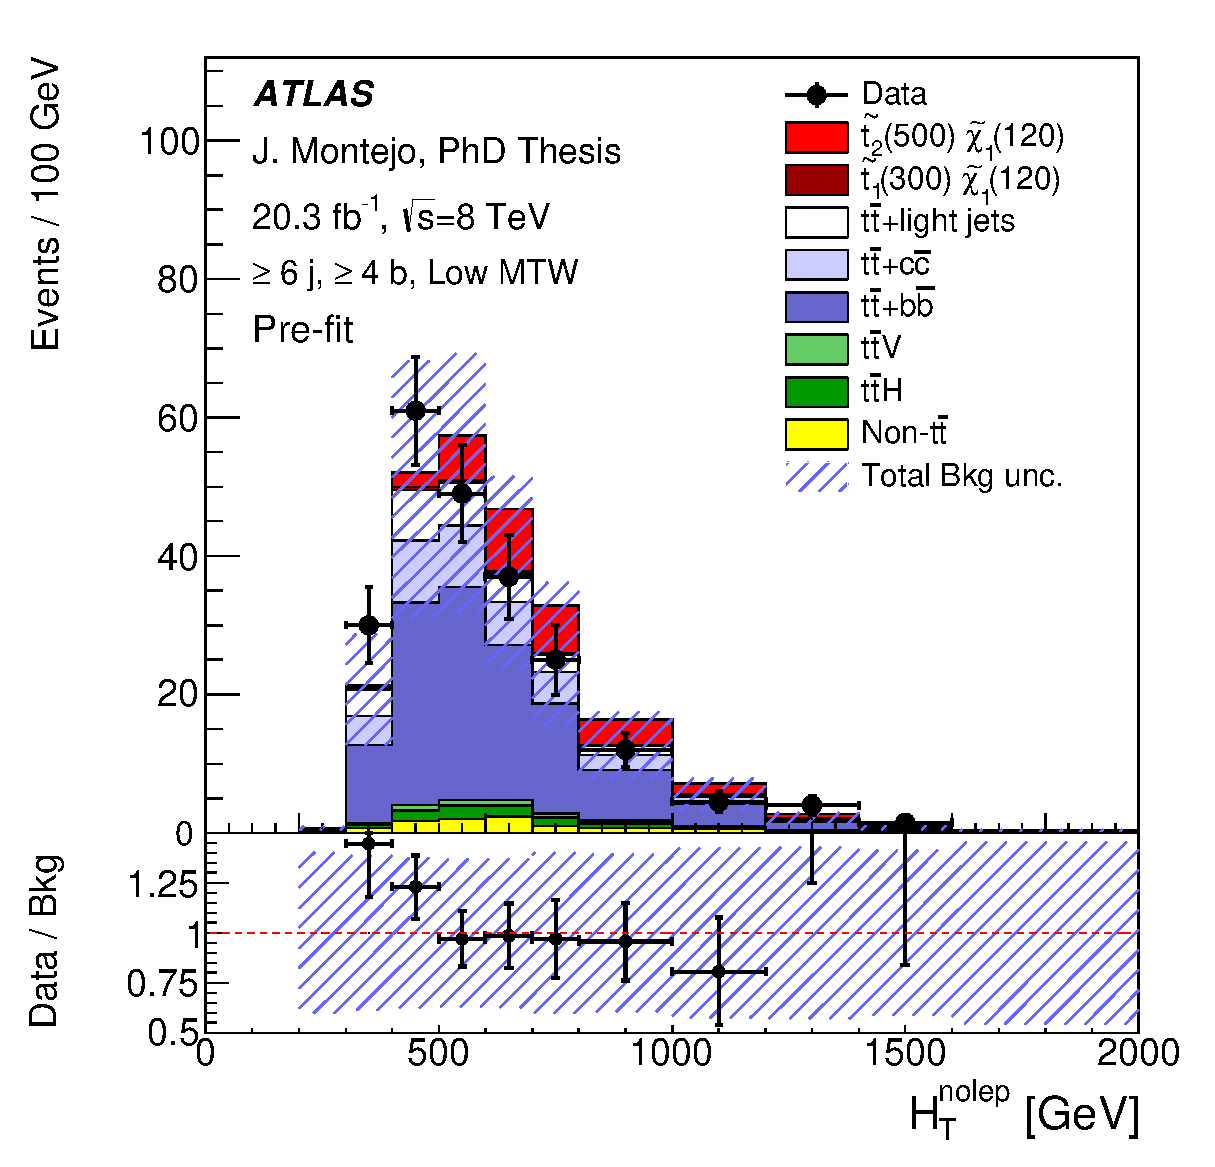
\includegraphics[width=0.41\textwidth]{Analysis/Figures_stop2/Prefit_HTnolep_unblind//HTnolep_6jetin4btaginLowMTW8TeV.eps} 
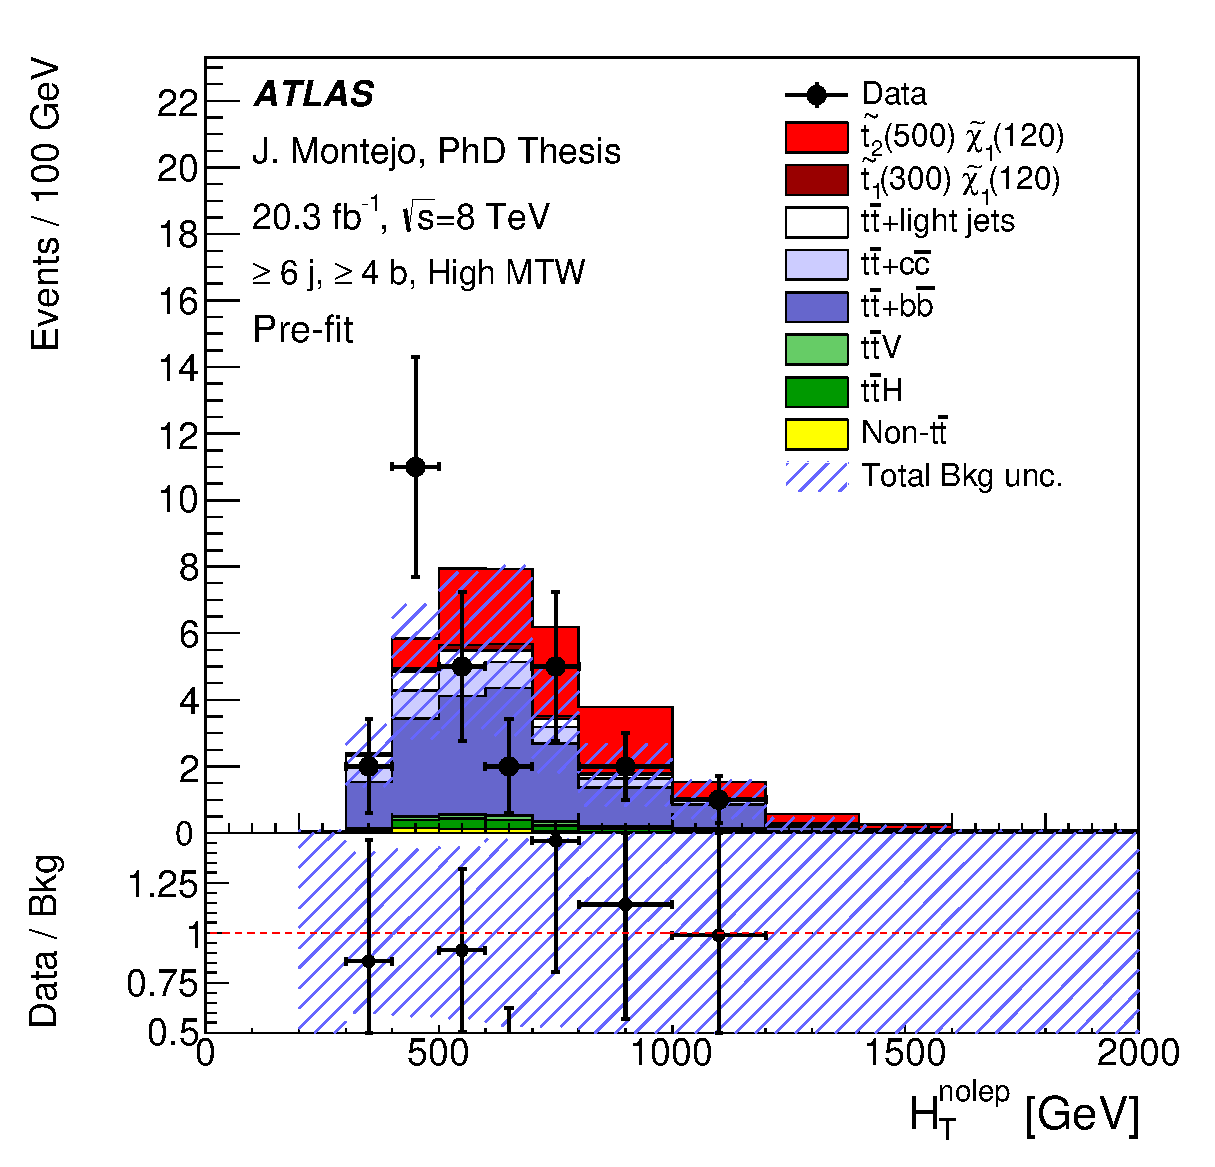
\includegraphics[width=0.41\textwidth]{Analysis/Figures_stop2/Prefit_HTnolep_unblind//HTnolep_6jetin4btaginHighMTW8TeV.eps} \\
\caption{
Comparison of the $\htnol$ distribution between data and prediction in each of the
channels considered in the analysis before the fit to data: $\geq 6$ jets/2 $b$-tags (top), $\geq 6$ jets/3 $b$-tags (middle) and
$\geq 6$ jets/$\geq 4$ $b$-tags (bottom), separately for ``low $\mtw$'' (left) and ``high $\mtw$'' (right).
The expected signal contributions from $\st_2\bar{\st}_2$ and $\st_1\bar{\st}_1$ production,
assuming $m_{\st_2}=500\gev$, $m_{\st_1}=300\gev$, $m_{\neut}=120\gev$ and BR$(\st_2 \to H\st_1)=1$, are also shown both
absolutely normalized and added to the stack (filled red histogram) and normalized to the background sum to compare the shape (open red histogram).
The total background prediction and uncertainties (shaded area), including statistical and total systematic contributions, are pre-fit. The last bin in all figures contains the overflow.}
\label{fig:HTnolep_prefit}
\end{center}
\end{figure}
%%%%%%%%%%%%%%


\begin{table}
\begin{center}
\begin{tabular}{l*{3}{c}}
\toprule
\toprule
 & \begin{tabular}{@{}c@{}}$\geq$ 6 j, 2 b\\ $\mtw < 120\gev$\end{tabular} & \begin{tabular}{@{}c@{}}$\geq$ 6 j, 3 b\\ $\mtw<120\gev$\end{tabular} & \begin{tabular}{@{}c@{}}$\geq$ 6 j, $\geq$ 4 b\\ $\mtw < 120\gev$\end{tabular} \\

\midrule
$\st_2\bar{\st}_2$&$47.6 \pm 2.0$&$45.5 \pm 1.8$&$37.1 \pm 3.6$\\
$\st_1\bar{\st}_1$&$220 \pm 54$&$29.5 \pm 7.5$&$1.76 \pm 0.5$\\
\midrule                                                                                    
$t\bar{t}+$light-jets &$9700 \pm 2400$&$1030 \pm 280$&$28 \pm 11$\\
$t\bar{t}+c\bar{c}$&$2000 \pm 1100$&$460 \pm 270$&$40 \pm 24$\\
$t\bar{t}+b\bar{b}$&$780 \pm 430$&$530 \pm 290$&$134 \pm 72$\\
$t\bar{t}V$&$101 \pm 33$&$24.8 \pm 8.1$&$4.8 \pm 1.6$\\
$t\bar{t}H$&$37.1 \pm 3.2$&$22.6 \pm 2.2$&$9.0 \pm 1.2$\\
$W$+jets &$430 \pm 300$&$47 \pm 32$&$3.5 \pm 2.4$\\
$Z$+jets &$50 \pm 24$&$5.5 \pm 2.4$&$0.41 \pm 0.29$\\
Single top &$457 \pm 75$&$67 \pm 12$&$6.4 \pm 1.5$\\
Diboson &$25.8 \pm 9.0$&$3.4 \pm 1.3$&$0.28 \pm 0.13$\\
Multijet &$9.2 \pm 3.5$&$2.17 \pm 0.97$&$0.84 \pm 0.34$\\
\midrule                                                                                      
Total background &$13500 \pm 3200$&$2190 \pm 580$&$228 \pm 84$\\
\midrule                                                                                      
Data                  &  $13433$                 & $2411$                & $246$               \\
\bottomrule
\bottomrule
\end{tabular}
\vspace{1cm}

\begin{tabular}{l*{3}{c}}
\toprule
\toprule
 & \begin{tabular}{@{}c@{}}$\geq$ 6 j, 2 b\\ $\mtw \geq 120\gev$\end{tabular} & \begin{tabular}{@{}c@{}}$\geq$ 6 j, 3 b\\ $\mtw \geq 120\gev$\end{tabular} & \begin{tabular}{@{}c@{}}$\geq$ 6 j, $\geq$ 4 b\\ $\mtw \geq 120\gev$\end{tabular} \\
 \midrule
$\st_2\bar{\st}_2$&$18.6 \pm 0.97$&$17.4 \pm 0.96$&$14.2 \pm 1.7$\\
$\st_1\bar{\st}_1$&$68 \pm 17$&$10.1 \pm 2.6$&$0.69 \pm 0.21$\\
\midrule                                                                                
$t\bar{t}+$light-jets &$920 \pm 320$&$88 \pm 33$&$2.34 \pm 0.79$\\
$t\bar{t}+c\bar{c}$&$220 \pm 130$&$51 \pm 29$&$4.4 \pm 2.6$\\
$t\bar{t}+b\bar{b}$&$95 \pm 55$&$68 \pm 38$&$18 \pm 10$\\
$t\bar{t}V$&$20.1 \pm 6.4$&$4.6 \pm 1.5$&$0.82 \pm 0.27$\\
$t\bar{t}H$&$6.26 \pm 0.62$&$3.55 \pm 0.4$&$1.42 \pm 0.21$\\
$W$+jets &$49 \pm 34$&$4.7 \pm 3.3$&$0.17 \pm 0.17$\\
$Z$+jets &$13.0 \pm 6.2$&$1.07 \pm 0.49$&$0.05 \pm 0.05$\\
Single top &$48 \pm 10$&$6.6 \pm 2.4$&$0.42 \pm 0.14$\\
Diboson &$3.4 \pm 1.2$&$0.38 \pm 0.17$&$0.03 \pm 0.02$\\
Multijet &$0.00 \pm 0.00$&$0.00 \pm 0.00$&$0.00 \pm 0.00$\\
\midrule                                                                                
Total background &$1380 \pm 400$&$228 \pm 70$&$28 \pm 12$\\
\midrule                                                                                
Data                  & $1495$                &  $281$             & $31$                \\
\bottomrule
\bottomrule
\end{tabular}
%%\\

%
\end{center}
\caption{
Pre-fit event yields for signal and backgrounds in each of the analysis regions.
The expected signal contributions from $\st_2\bar{\st}_2$ and $\st_1\bar{\st}_1$ production,
assuming $m_{\st_2}=500\gev$, $m_{\st_1}=300\gev$, $m_{\neut}=120\gev$ and BR$(\st_2 \to H\st_1)=1$, are also shown.
The quoted uncertainties are the sum in quadrature of the statistical and
total systematic uncertainties on the yields. 
}
\label{tab:Prefit_Yields_stop2}
\end{table}
 


\subsection{Fit results}
A fit to the data is performed under the background-only hypothesis, and the fitted NPs are shown in figure~\ref{fig:Stop2_fit}.
The corresponding correlation matrix for the
fitted NPs can be found in figure~\ref{fig:corrmat_Stop2}.

\begin{figure}[!tp]
\begin{center}
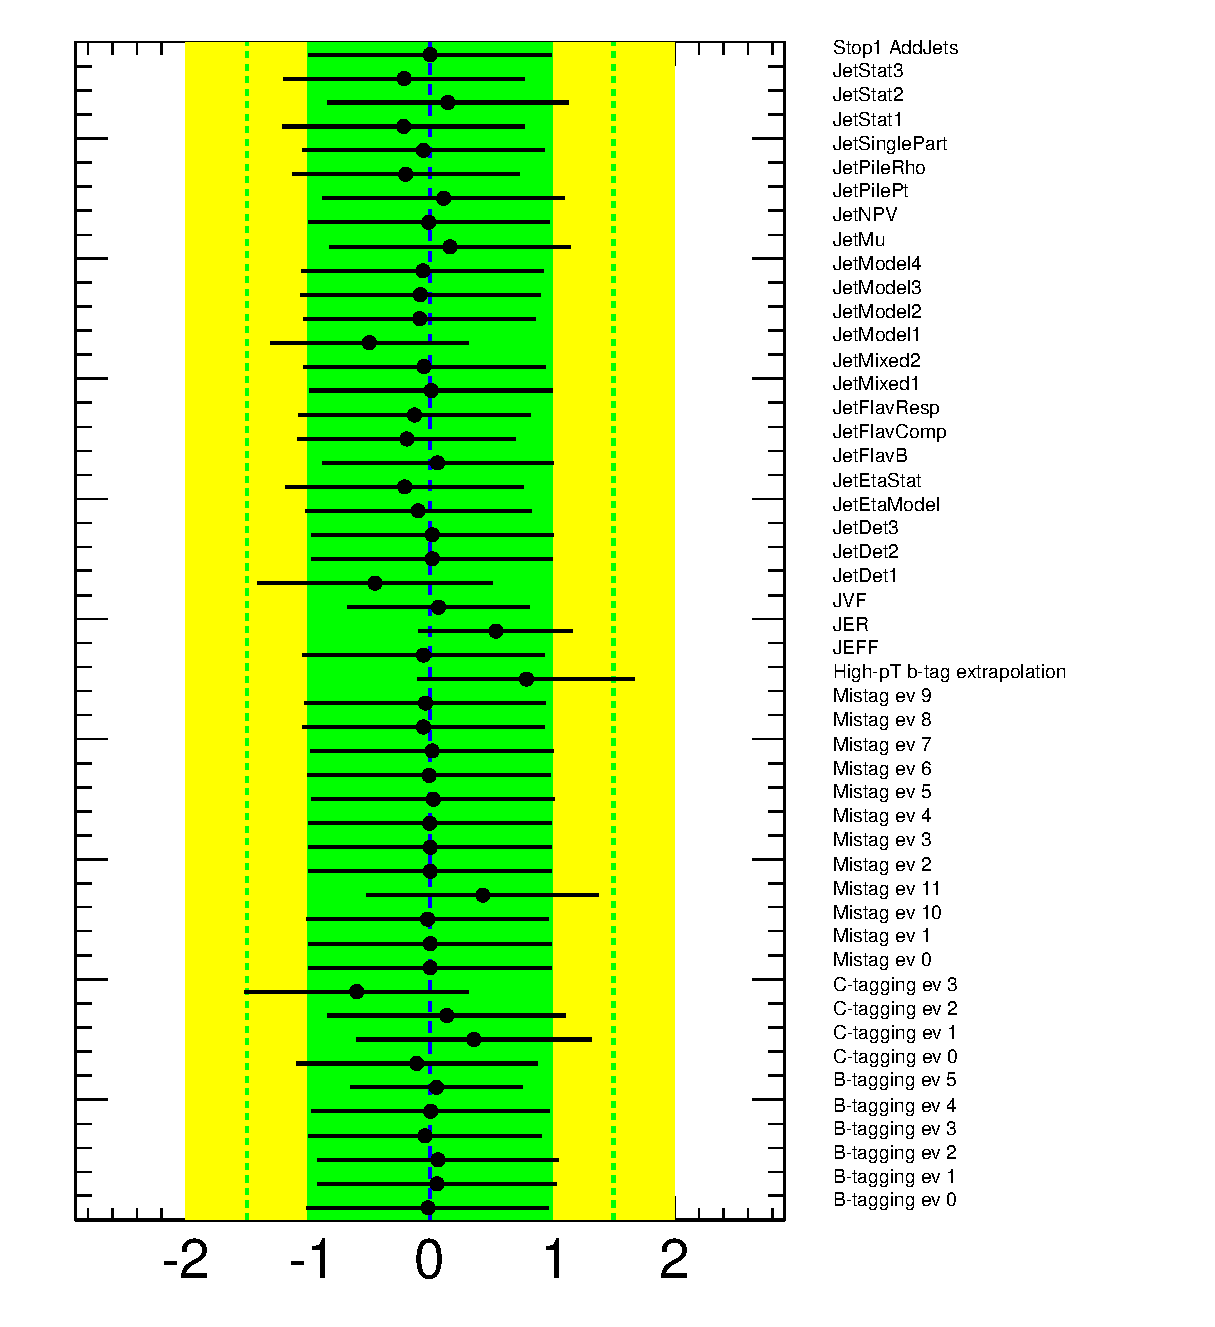
\includegraphics[trim=0cm 0cm 1.5cm 0cm, clip=true, width=0.49\textwidth]{Analysis/Figures_stop2/detectorUNCtesis_stop2.eps}
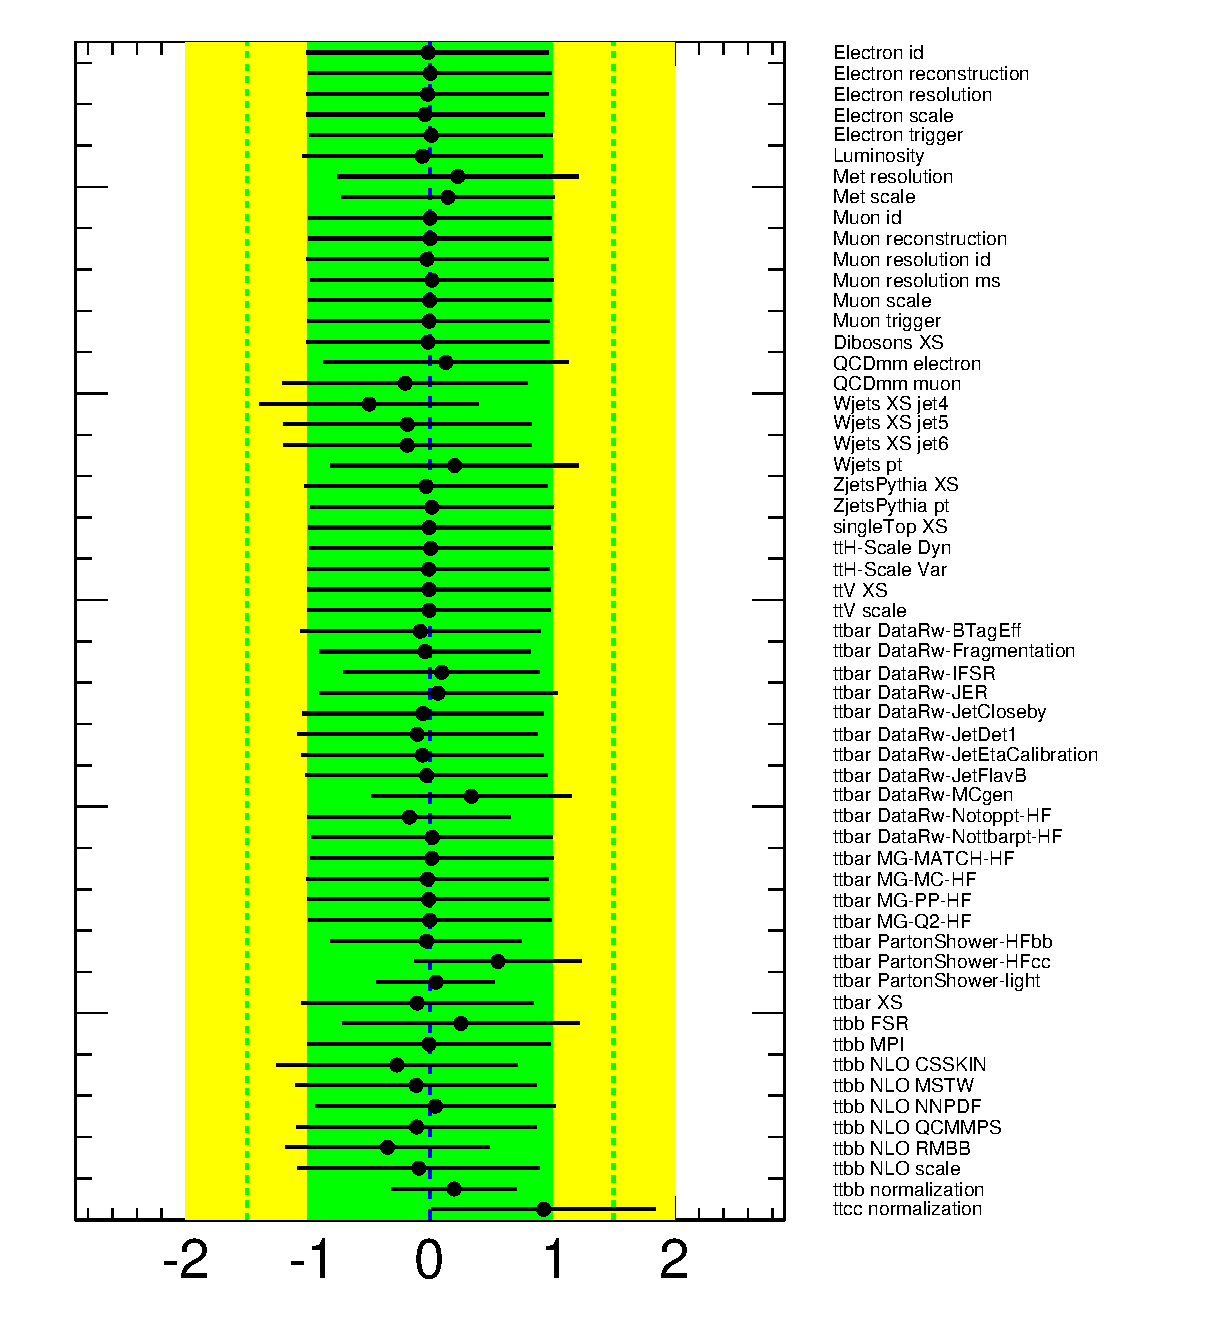
\includegraphics[trim=0cm 0cm 1.5cm 0cm, clip=true, width=0.49\textwidth]{Analysis/Figures_stop2/otherUNCtesis_stop2.eps}
\caption{Fitted NPs under the background-only hypothesis. A detailed description of the naming of the NP can be found in appendix~\ref{app:glossary}.}
\label{fig:Stop2_fit} 
\end{center}
\begin{center}
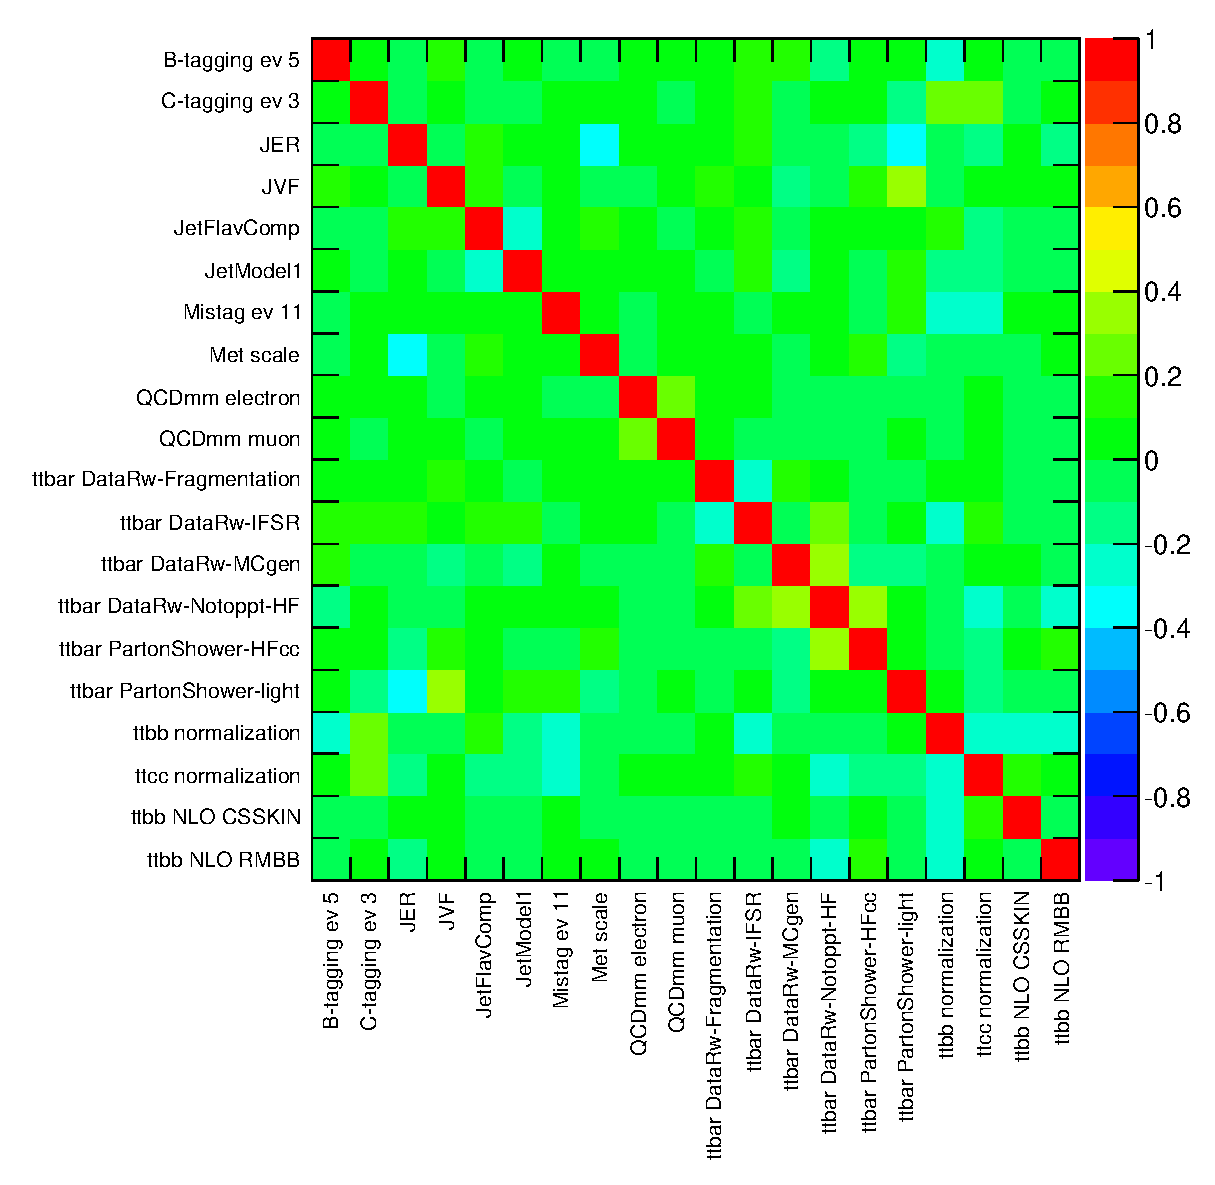
\includegraphics[width=0.49\textwidth]{Analysis/Figures_stop2/CorrMat_stop2.eps}
\caption{Correlation matrix corresponding to the fit under the background-only hypothesis.
Only NPs with a correlation coefficient of at least 20\% with any other parameter are displayed.}
\label{fig:corrmat_Stop2} 
\end{center}
\end{figure}

Given that only regions with $\geq 6$ jets are considered, much smaller pulls and constrains are expected than in the \ttH\ or $\TT$ analyses. 
The NPs that show significant pulls or constrains have already been discussed in section~\ref{subsec:fit_ttH}.
A further validation of the fit can be performed by comparing the fit result from the three analyses as shown in figure~\ref{fig:fit_three}. Although the fits are not statistically independent since a large overlap of the data samples exist, it is a good validation to confirm that the main features are present in the three analyses, even if the selection cuts, event categorization and discriminant variable are different among them.

\begin{figure}[!tp]
\begin{center}
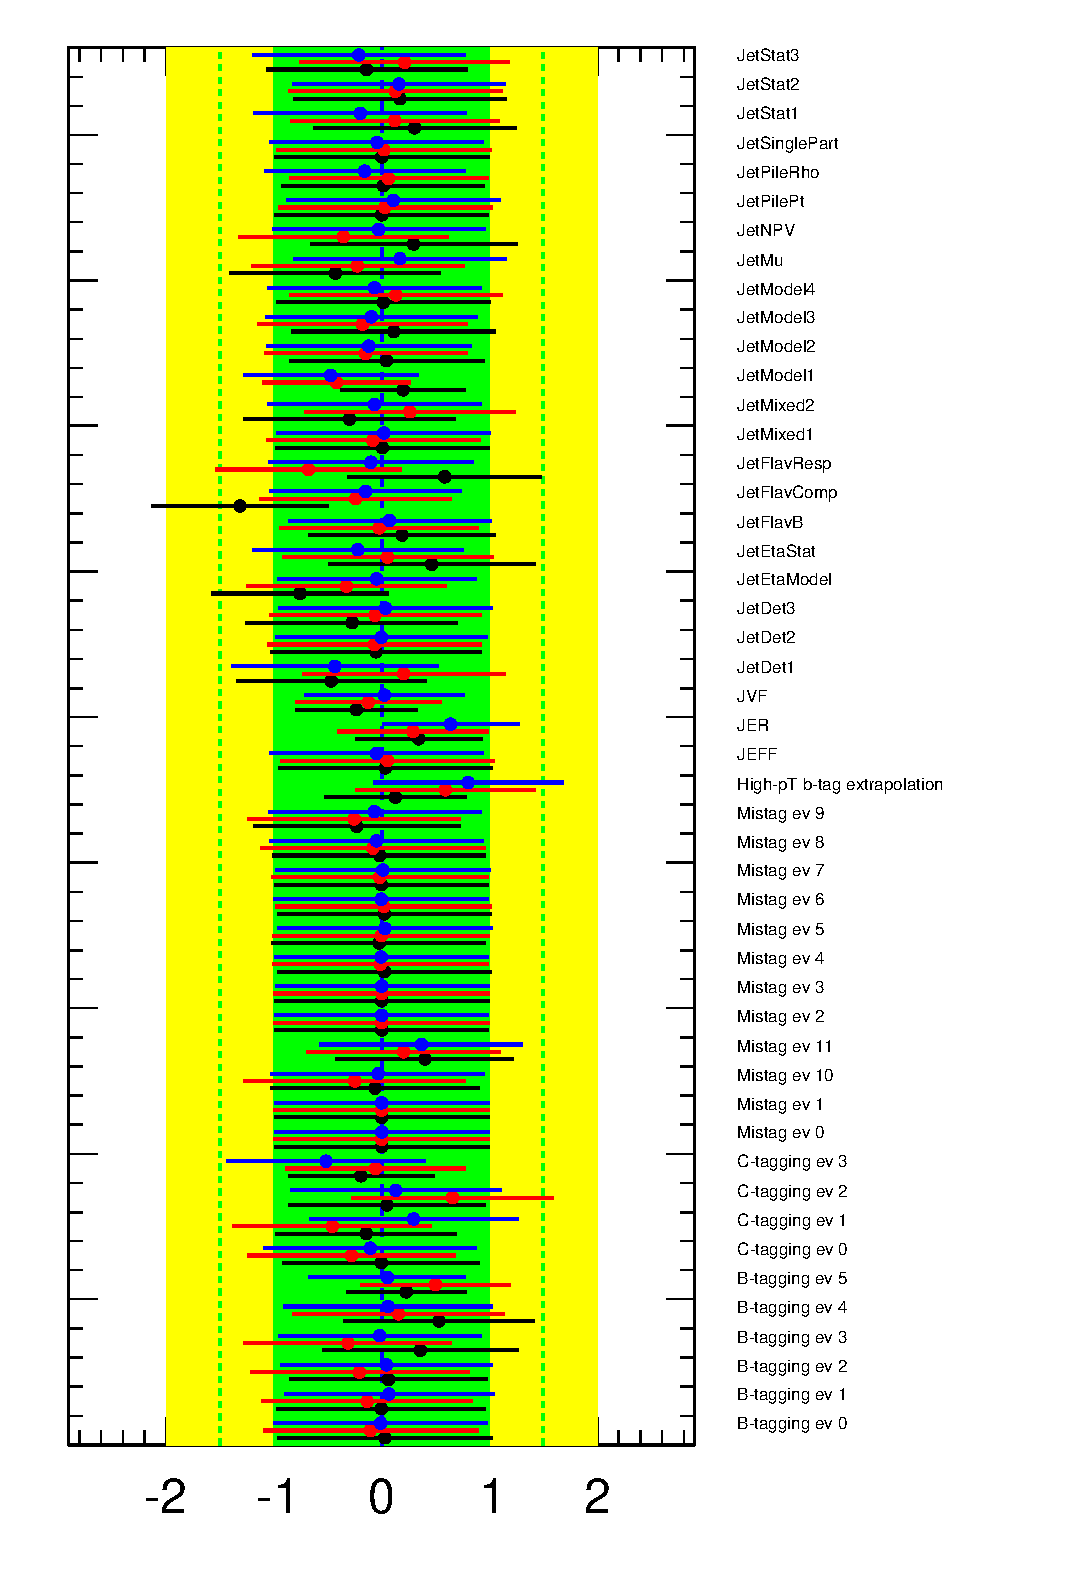
\includegraphics[trim=0cm 0cm 1.5cm 0cm, clip=true, width=0.49\textwidth]{Analysis/Figures_stop2/detectorUNCthreeanalyses.eps}
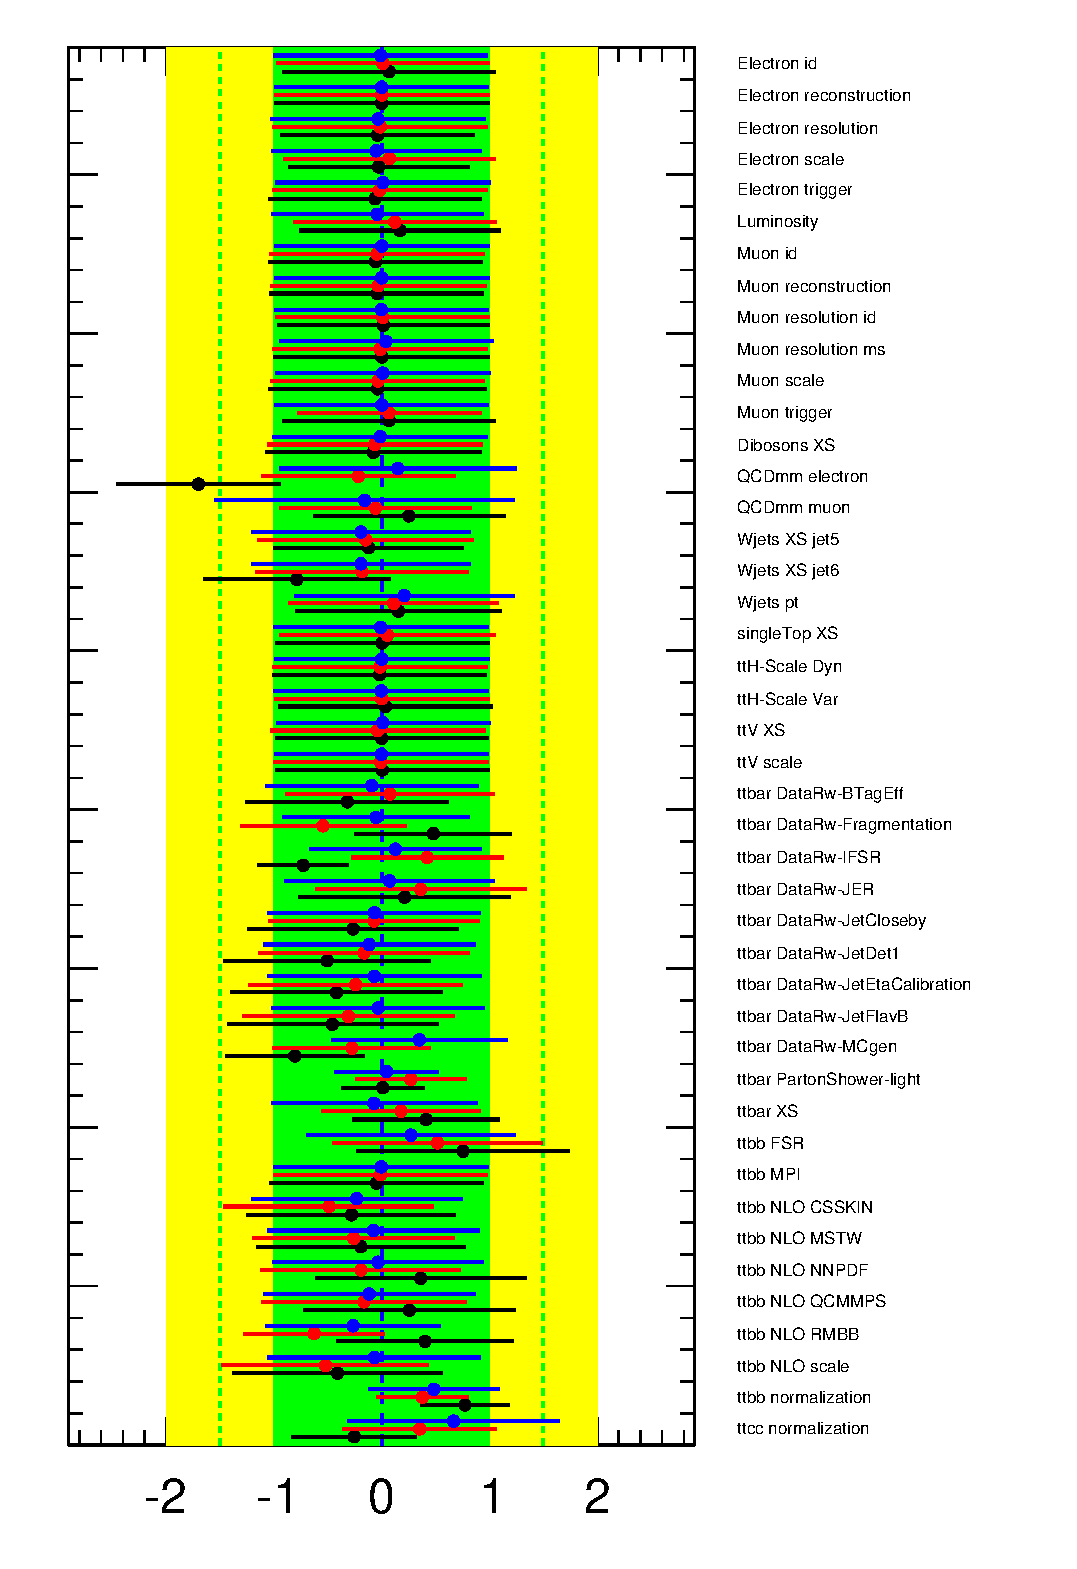
\includegraphics[trim=0cm 0cm 1.5cm 0cm, clip=true, width=0.49\textwidth]{Analysis/Figures_stop2/otherUNCthreeanalyses.eps}
\caption{Fitted NPs under the background-only hypothesis for the three analyses (blue) \ttH, (red) $\TT$ and (black) $\stoptwobar$.}
\label{fig:fit_three} 
\end{center}
\end{figure}

Figure~\ref{fig:postfit_Stop2} shows the comparison of data and prediction for the $\htnol$ distributions 
in each of the regions considered, after the fit to data. 
Compared to the pre-fit distributions, the total background uncertainty is significantly
reduced after the fit, resulting in an increase in the search sensitivity.
The corresponding post-fit yields can be found in table~\ref{tab:Postfit_Yields_stop2}.

\begin{figure}[!tp]
\begin{center}
{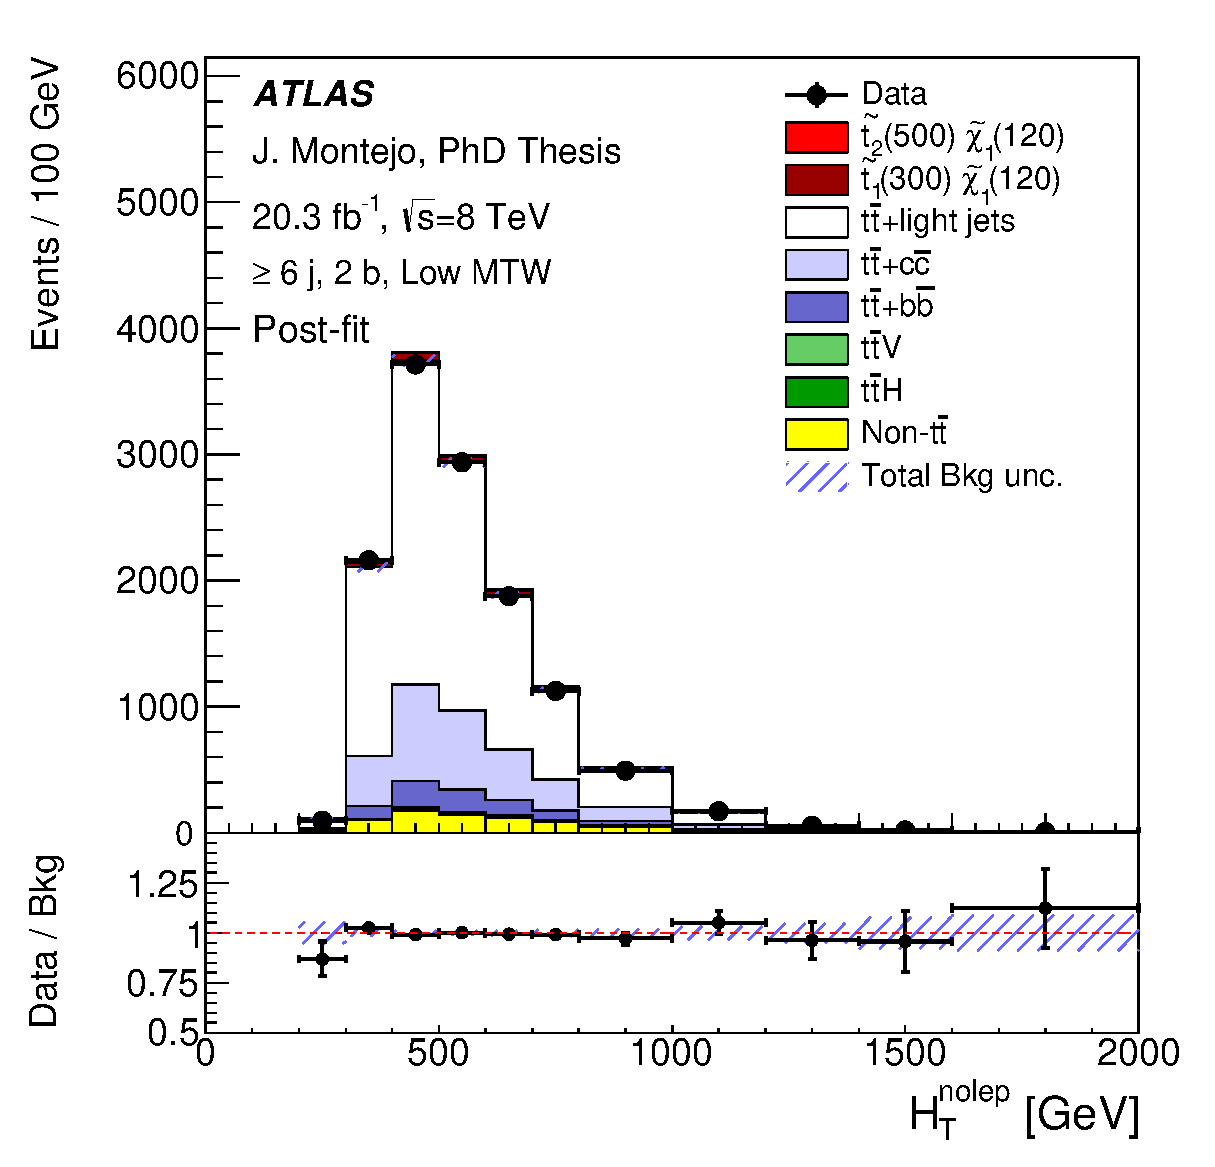
\includegraphics[width=0.41\textwidth]{Analysis/Figures_stop2/Postfit_HTnolep_unblind/HTnolep_6jetin2btagexLowMTW8TeV.eps}}
{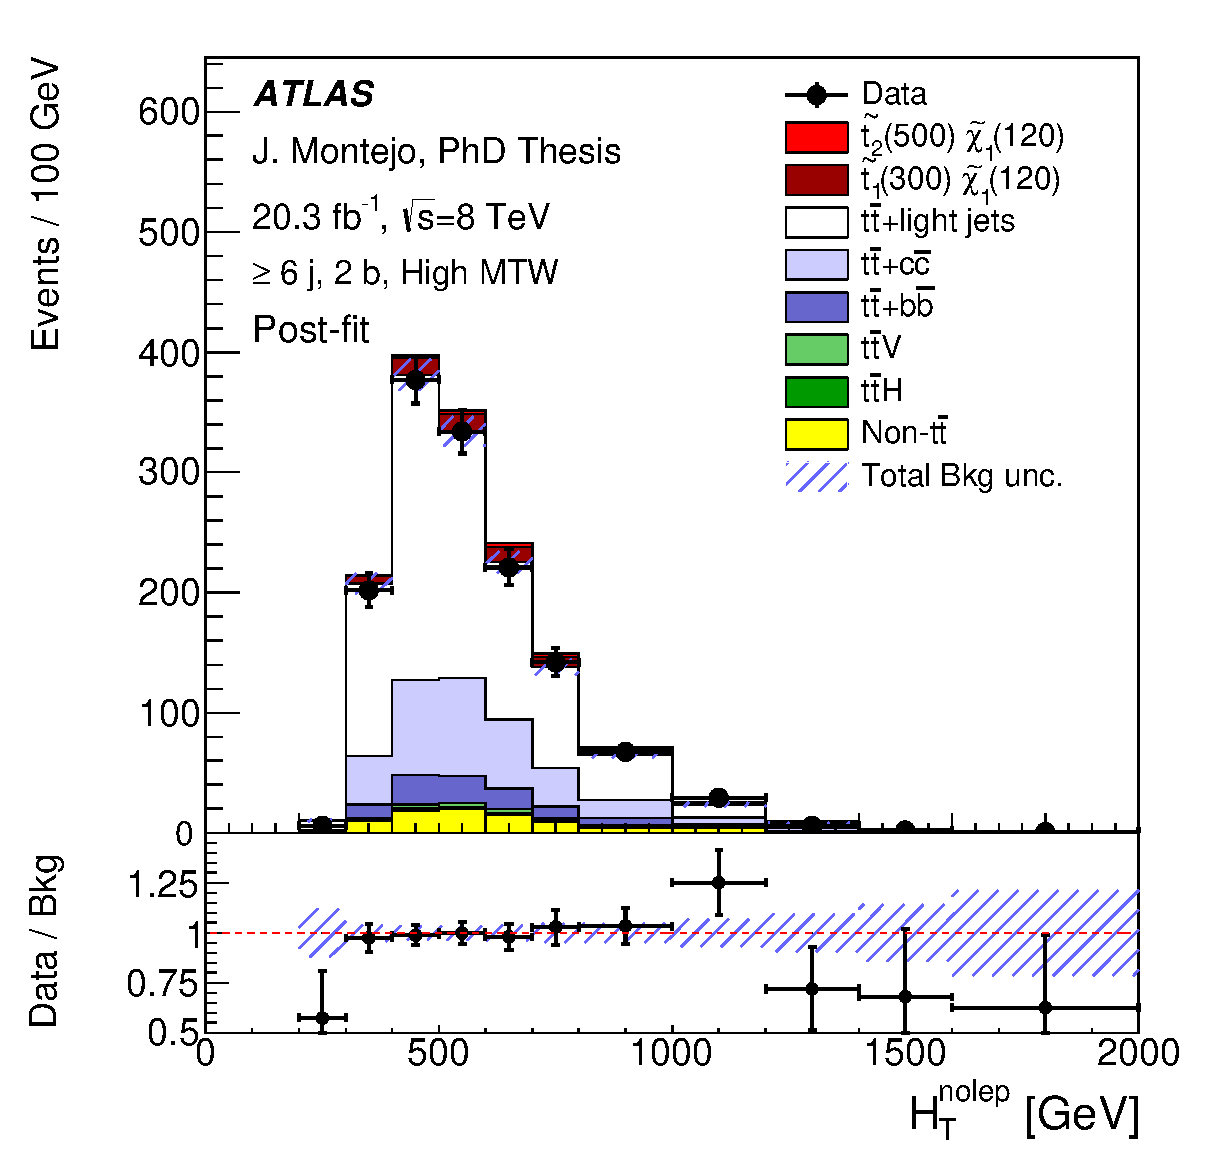
\includegraphics[width=0.41\textwidth]{Analysis/Figures_stop2/Postfit_HTnolep_unblind/HTnolep_6jetin2btagexHighMTW8TeV.eps}} \\
{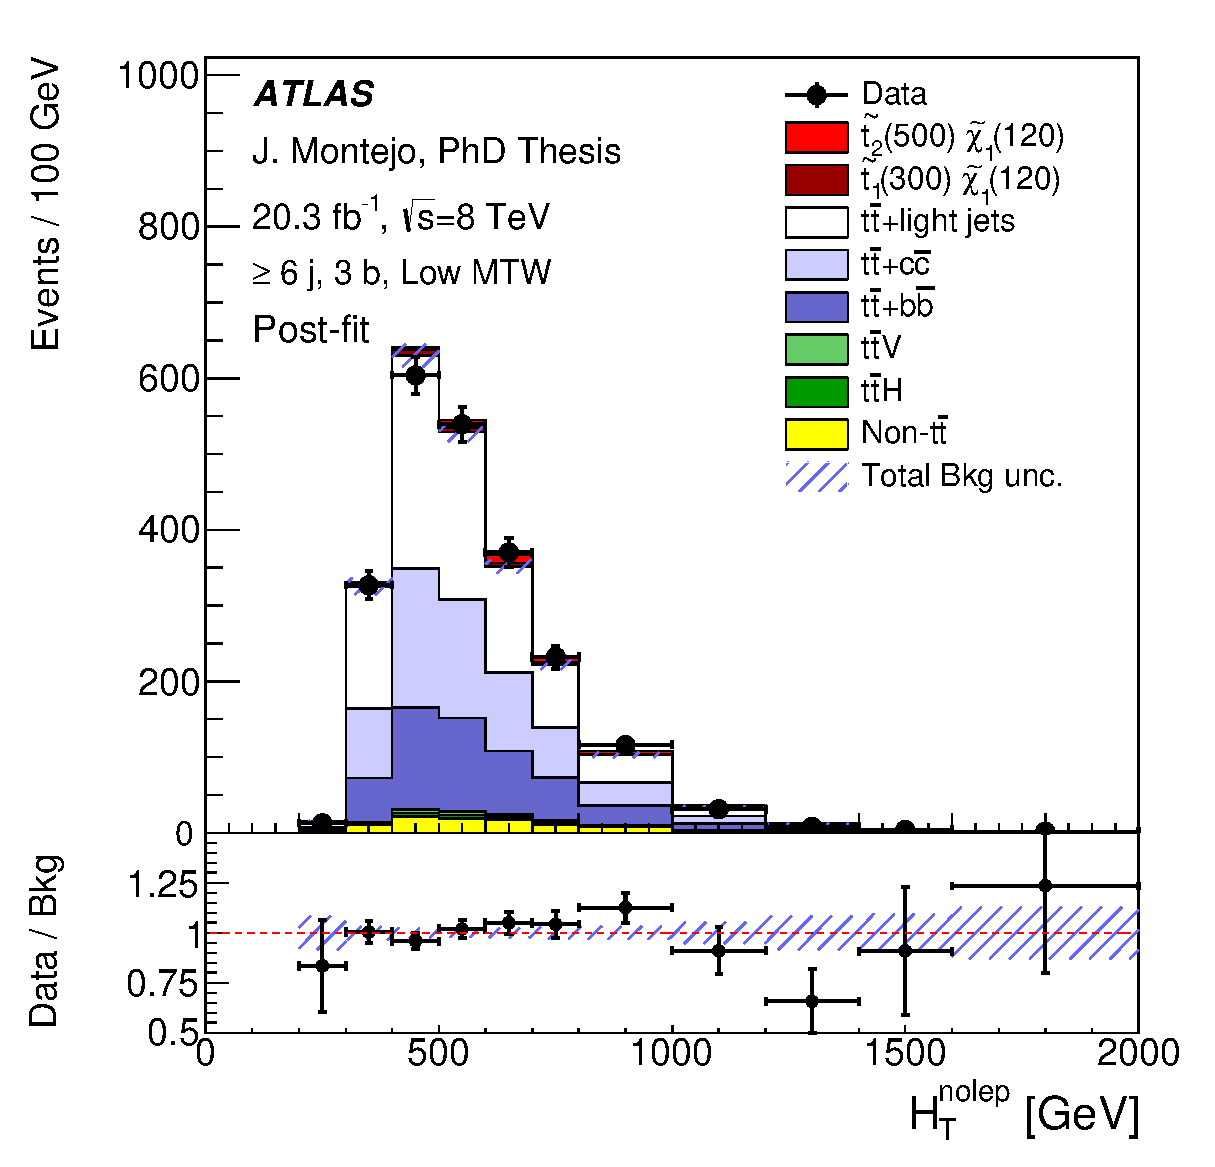
\includegraphics[width=0.41\textwidth]{Analysis/Figures_stop2/Postfit_HTnolep_unblind/HTnolep_6jetin3btagexLowMTW8TeV.eps}} 
{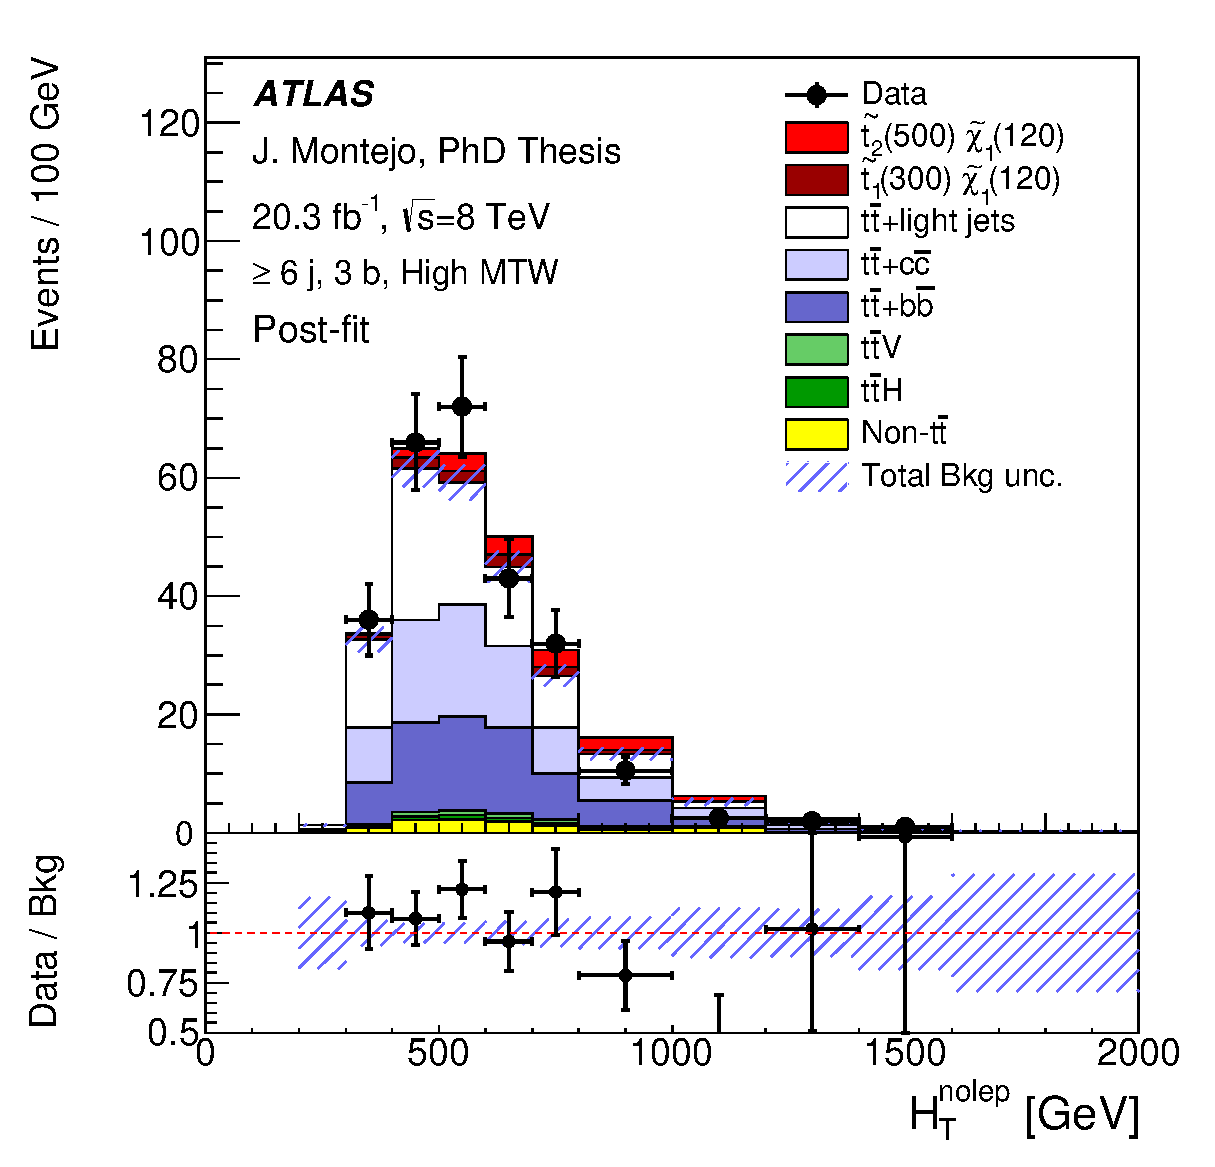
\includegraphics[width=0.41\textwidth]{Analysis/Figures_stop2/Postfit_HTnolep_unblind/HTnolep_6jetin3btagexHighMTW8TeV.eps}} \\
{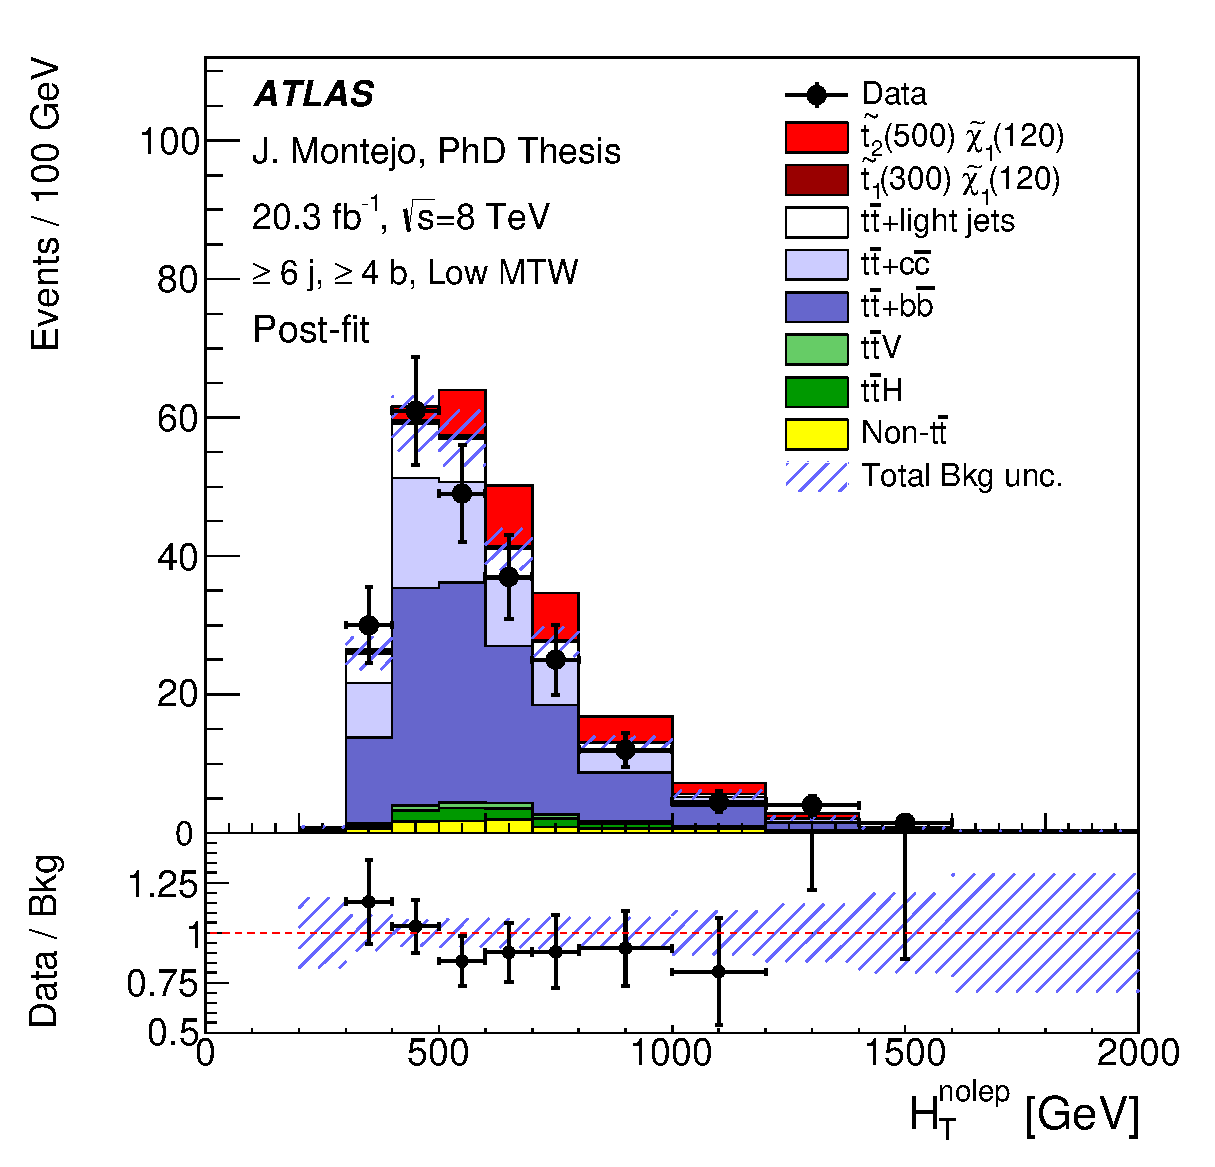
\includegraphics[width=0.41\textwidth]{Analysis/Figures_stop2/Postfit_HTnolep_unblind/HTnolep_6jetin4btaginLowMTW8TeV.eps}} 
{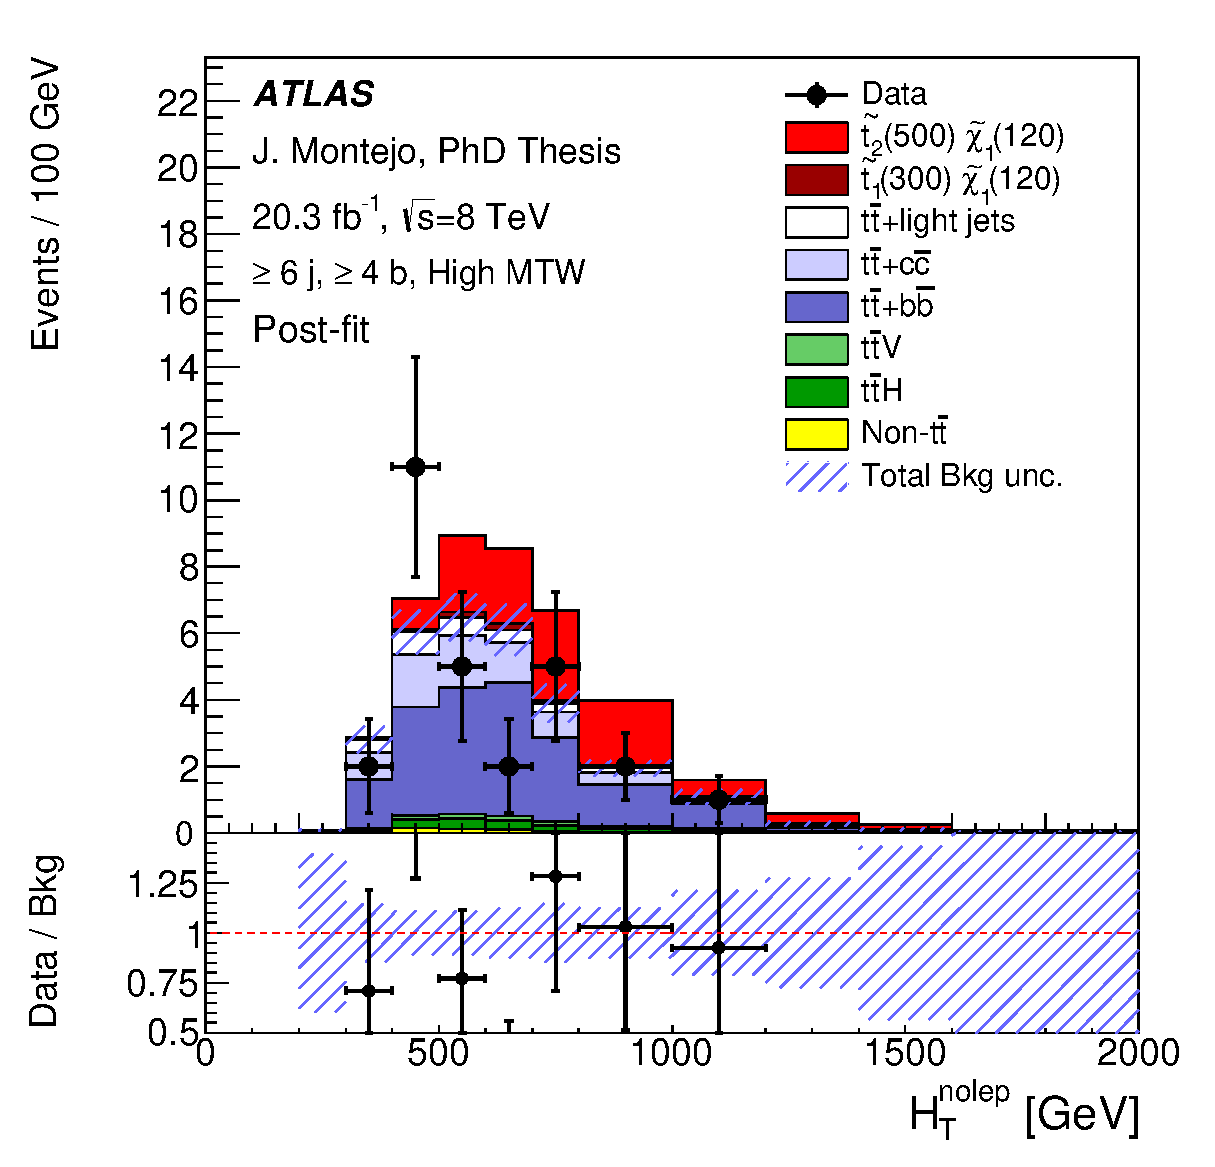
\includegraphics[width=0.41\textwidth]{Analysis/Figures_stop2/Postfit_HTnolep_unblind/HTnolep_6jetin4btaginHighMTW8TeV.eps}} \\
\caption{
Comparison of the $\htnol$ distribution between data and prediction in each of the
channels considered in the analysis after the fit to data: $\geq 6$ jets/2 $b$-tags (top), $\geq 6$ jets/3 $b$-tags (middle) and
$\geq 6$ jets/$\geq 4$ $b$-tags (bottom), separately for ``low $\mtw$'' (left) and ``high $\mtw$'' (right).
The expected signal contributions from $\st_2\bar{\st}_2$ and $\st_1\bar{\st}_1$ production,
assuming $m_{\st_2}=500\gev$, $m_{\st_1}=300\gev$, $m_{\neut}=120\gev$ and BR$(\st_2 \to H\st_1)=1$, are also shown both
absolutely normalized and added to the stack (filled red histogram) and normalized to the background sum to compare the shape (open red histogram).
The total background prediction and uncertainties (shaded area), including statistical and total systematic contributions, are post-fit. The last bin in all figures contains the overflow.
}
\label{fig:postfit_Stop2} 
\end{center}
\end{figure}


\begin{table}
\begin{center}
\begin{tabular}{l*{3}{c}}
\toprule
\toprule
 & \begin{tabular}{@{}c@{}}$\geq$ 6 j, 2 b\\ $\mtw < 120\gev$\end{tabular} & \begin{tabular}{@{}c@{}}$\geq$ 6 j, 3 b\\ $\mtw<120\gev$\end{tabular} & \begin{tabular}{@{}c@{}}$\geq$ 6 j, $\geq$ 4 b\\ $\mtw < 120\gev$\end{tabular} \\

\midrule
$t\bar{t}+$light-jets &$8940 \pm 740$&$1000 \pm 130$&$29.5 \pm 7.5$\\
$t\bar{t}+c\bar{c}$&$2800 \pm 860$&$700 \pm 200$&$65 \pm 18$\\
$t\bar{t}+b\bar{b}$&$790 \pm 200$&$540 \pm 120$&$138 \pm 26$\\
$t\bar{t}V$&$93 \pm 29$&$23.6 \pm 7.4$&$4.6 \pm 1.4$\\
$t\bar{t}H$&$35.5 \pm 2.0$&$21.7 \pm 1.4$&$8.65 \pm 0.77$\\
$W$+jets &$270 \pm 160$&$30 \pm 18$&$2.2 \pm 1.4$\\
$Z$+jets &$54 \pm 20$&$5.8 \pm 2.2$&$0.53 \pm 0.28$\\
Single top &$435 \pm 46$&$65.8 \pm 8.0$&$6.5 \pm 1.1$\\
Diboson &$24.2 \pm 7.7$&$3.4 \pm 1.2$&$0.26 \pm 0.11$\\
Multijet &$8.7 \pm 3.3$&$2.4 \pm 1.0$&$0.78 \pm 0.31$\\
\midrule                                                                                           
Total background &$13500 \pm 120$&$2390 \pm 46$&$256 \pm 14$\\
\midrule                                                                                          
Data                  & $13433$                & $2411$               & $246$               \\
\bottomrule
\bottomrule
\end{tabular}
\vspace{1cm}

\begin{tabular}{l*{3}{c}}
\toprule
\toprule
 & \begin{tabular}{@{}c@{}}$\geq$ 6 j, 2 b\\ $\mtw \geq 120\gev$\end{tabular} & \begin{tabular}{@{}c@{}}$\geq$ 6 j, 3 b\\ $\mtw \geq 120\gev$\end{tabular} & \begin{tabular}{@{}c@{}}$\geq$ 6 j, $\geq$ 4 b\\ $\mtw \geq 120\gev$\end{tabular} \\
 \midrule
$t\bar{t}+$light-jets &$936 \pm 97$&$96 \pm 15$&$2.69 \pm 0.69$\\
$t\bar{t}+c\bar{c}$&$340 \pm 110$&$81 \pm 24$&$7.2 \pm 2.1$\\
$t\bar{t}+b\bar{b}$&$104 \pm 29$&$74 \pm 18$&$19.6 \pm 3.9$\\
$t\bar{t}V$&$19.3 \pm 6.0$&$4.6 \pm 1.4$&$0.83 \pm 0.27$\\
$t\bar{t}H$&$6.3 \pm 0.44$&$3.61 \pm 0.28$&$1.44 \pm 0.15$\\
$W$+jets &$30 \pm 18$&$3.1 \pm 2.0$&$0.14 \pm 0.12$\\
$Z$+jets &$13.9 \pm 5.2$&$0.96 \pm 0.4$&$0.05 \pm 0.04$\\
Single top &$47.4 \pm 7.0$&$7.1 \pm 1.6$&$0.42 \pm 0.11$\\
Diboson &$3.3 \pm 1.1$&$0.38 \pm 0.15$&$0.03 \pm 0.01$\\
Multijet &$0.00 \pm 0.00$&$0.00 \pm 0.00$&$0.00 \pm 0.00$\\
\midrule                                                                             
Total background &$1500 \pm 37$&$270 \pm 10$&$32.4 \pm 2.9$\\
\midrule                                                                            
Data                  & $1495$               & $281$              & $31$              \\
\bottomrule
\bottomrule
\end{tabular}
%%\\

%
\end{center}
\caption{
Post-fit event yields under the background-only hypothesis in each of the analysis regions.
The expected signal contributions from $\st_2\bar{\st}_2$ and $\st_1\bar{\st}_1$ production,
assuming $m_{\st_2}=500\gev$, $m_{\st_1}=300\gev$, $m_{\neut}=120\gev$ and BR$(\st_2 \to H\st_1)=1$, are also shown.
The quoted uncertainties are the sum in quadrature of the statistical and
total systematic uncertainties on the yields. 
}
\label{tab:Postfit_Yields_stop2}
\end{table}


\subsection{\texorpdfstring{Limits on $\stoptwobar$ production}{Limits on t2t2 production}}

The consistency of the data with the background prediction is assessed by 
computing the $p_0$-value for each signal scenario considered. 
The smallest $p_0$-value found, $0.0.5$, equivalent to a local significance
of $1.64$ standard deviations above the background-only prediction, is found to be at
BR$(\st_2 \to H \st_1)\sim 0.0$, BR$(\st_2 \to Z \st_1)\sim 0.3$ and BR$(\st_2 \to t \neut)\sim 0.7$
for $(m_{\st_2}, m_{\neut}) = (350, 20)\gev$.

In absence of a significant excess above the SM prediction, upper limits on the  $\st_2\bar{\st}_2$ production \xsec\ times branching ratio
are derived for the $\st_2$ simplified model.
Figure~\ref{fig:lim_2D_BrH1} shows the expected and observed limits in the $m_{\st_2}$--$m_{\neut}$ plane for the direct
$\st_2$ pair production simplified model with BR$(\st_2 \to H \st_1)=1$. 
The inclusion of $\stoponebar$ as signal improves the \xsec\ sensitivity by a maximum of 7\% for the lowest value of $m_{\st_1}$ considered.

Relaxing the assumption that BR$(\st_2 \to H \st_1)=1$, figure~\ref{fig:lim_triangle_BrScan} shows the exclusion limits as a function
of the $\st_2$ branching ratios for representative values of the masses of $\st_2$ and $\neut$. As expected, this search is particularly
sensitive to high BR$(\st_2 \to H \st_1)$.

\begin{figure}[tpb]
\centering
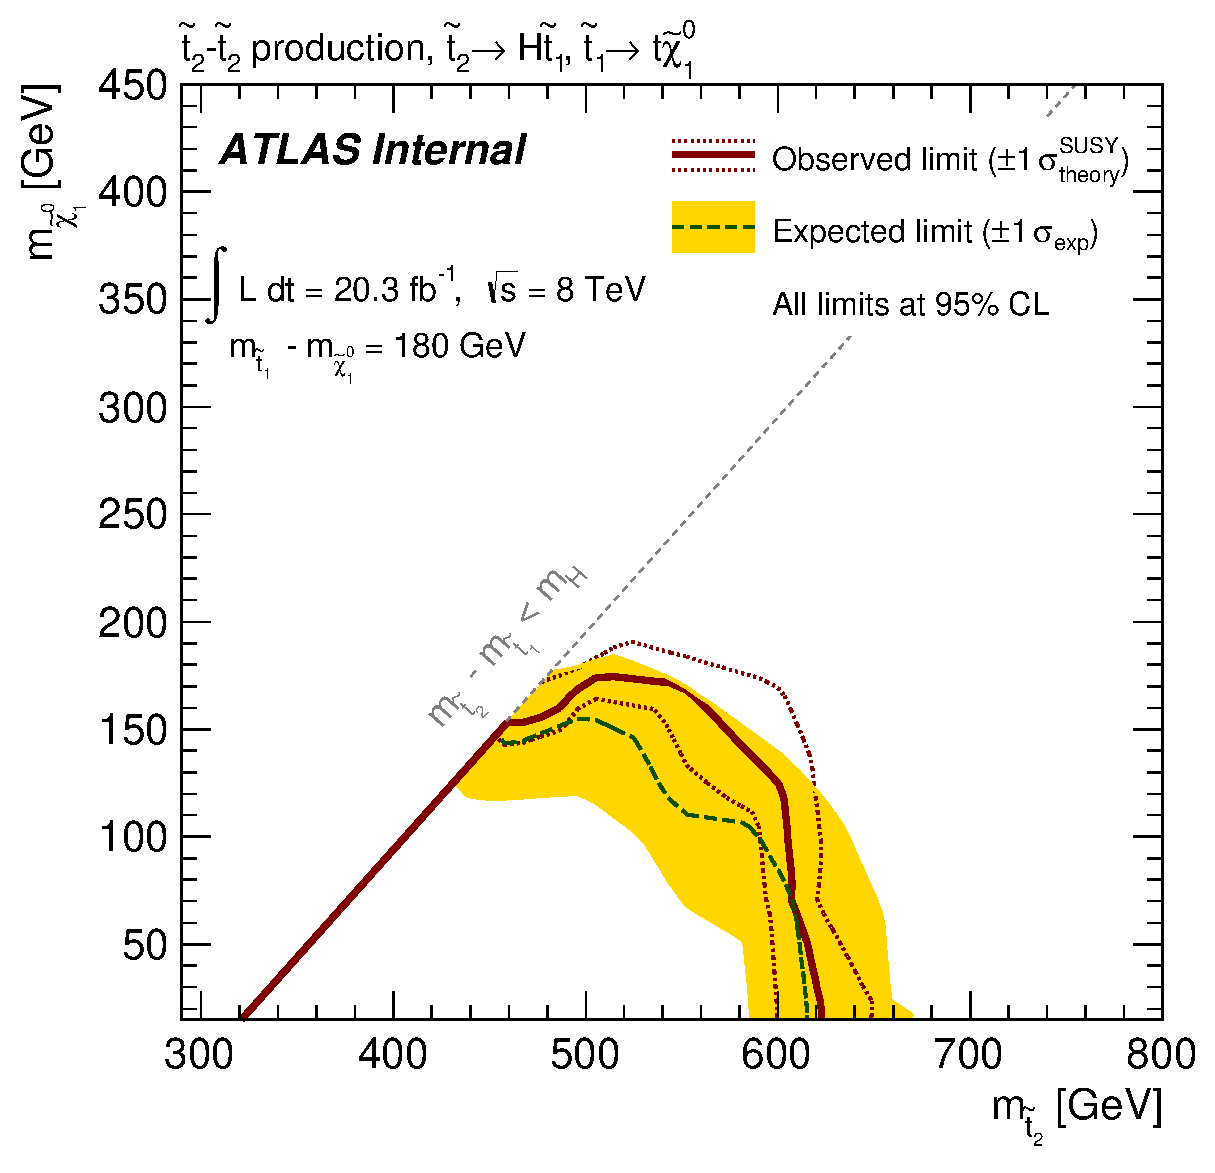
\includegraphics[width=0.7\textwidth]{Analysis/Figures_stop2/lim_2D_BrH1.eps}
\caption{
Expected and observed exclusion limits in the $m_{\st_2}$--$m_{\neut}$ plane for the direct
$\st_2$ pair production simplified model with BR$(\st_2 \to H \st_1)=1$.
The contours of the band around the expected limit are the $\pm 1$ s.d. results, including all uncertainties
except theoretical uncertainties on the signal cross
section. The dotted lines around the observed limit illustrate
the change in the observed limit as the nominal signal cross
section is scaled up and down by the theoretical uncertainty.
All limits are computed at 95\% CL.
\label{fig:lim_2D_BrH1}}
\end{figure}

\begin{figure}[tpb]
\centering
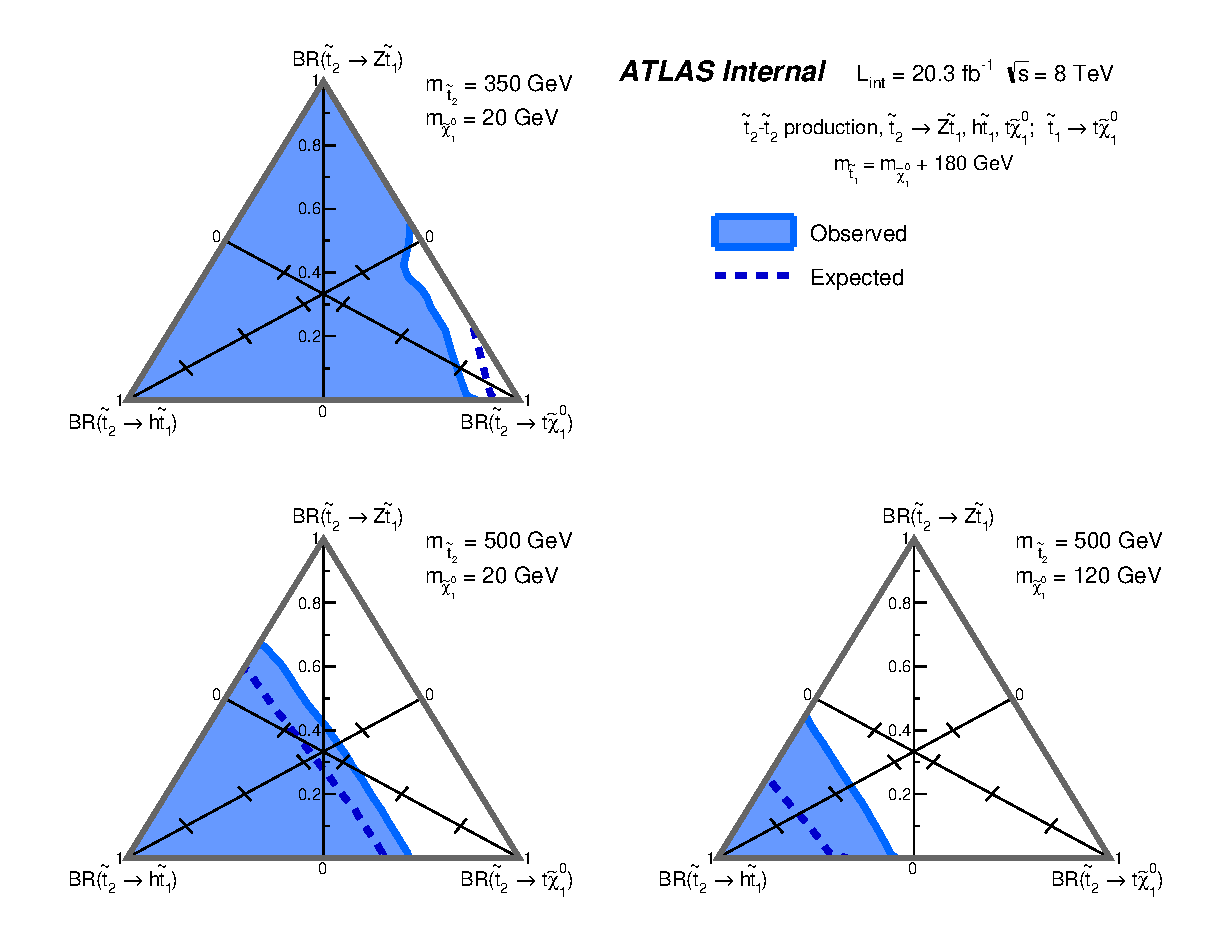
\includegraphics[width=0.9\textwidth]{Analysis/Figures_stop2/lim_triangle_BrScan.eps}
\caption{
Exclusion limits at 95\% CL are shown for the direct $\st_2$ pair production simplified model as a function of the branching
ratios BR$(\st_2 \to Z \st_1)$, BR$(\st_2 \to H \st_1)$ and BR$(\st_2 \to t \neut)$ for (top) $(m_{\st_2}, m_{\neut}) = (350, 20)\gev$,
(bottom left) $(500, 20)\gev$, and (bottom right) $(500, 120)\gev$.
The dashed and solid lines show the expected and observed limits, respectively, including all
uncertainties except the theoretical signal \xsec\ uncertainty (PDF and scale).
\label{fig:lim_triangle_BrScan}}
\end{figure}

\subsection{Comparison with other analyses}
The CMS collaboration has also published searches for $\stoptwobar$ production~\cite{Khachatryan:2014doa}, targeting the decay through a $Z$ boson or a Higgs boson. The exclusion limits are shown in figure~\ref{fig:CMS_stop2} assuming BR$(\st_2 \to H \st_1) = 1$. Limits are presented in the $m_{\st_2}$--$m_{\st_1}$ plane, a value of \unit[175]{\gev} has to be subtracted from the $y$-axis in order to compare to the ATLAS results.
The analysis presented here has better sensitivity than the single-lepton analysis, and comparable sensitivity to the full combination of the four analyses: single-lepton, opposite-sign dilepton, same-sign dilepton and trilepton. 

\begin{figure}[tpb]
  \begin{center}
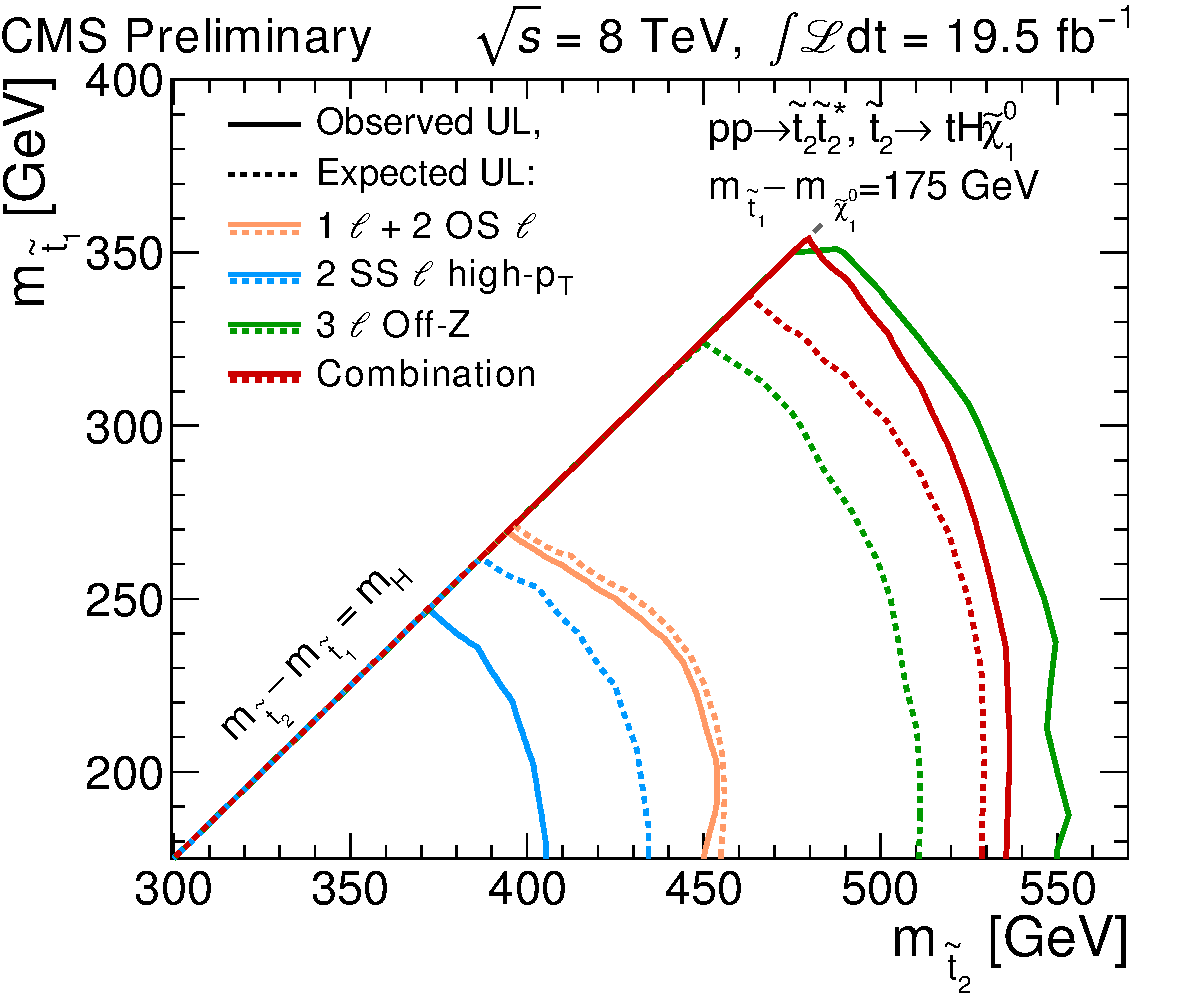
\includegraphics[width=0.6\textwidth]{Analysis/Figures_stop2/Figure_005-b.pdf}
  \caption{
Expected and observed exclusion limits in the $m_{\st_2}$--$m_{\neut}$ plane for the direct
$\st_2$ pair production simplified model with BR$(\st_2 \to H \st_1)=1$, from the CMS collaboration.
}
  \label{fig:CMS_stop2}
\end{center}
  \begin{center}
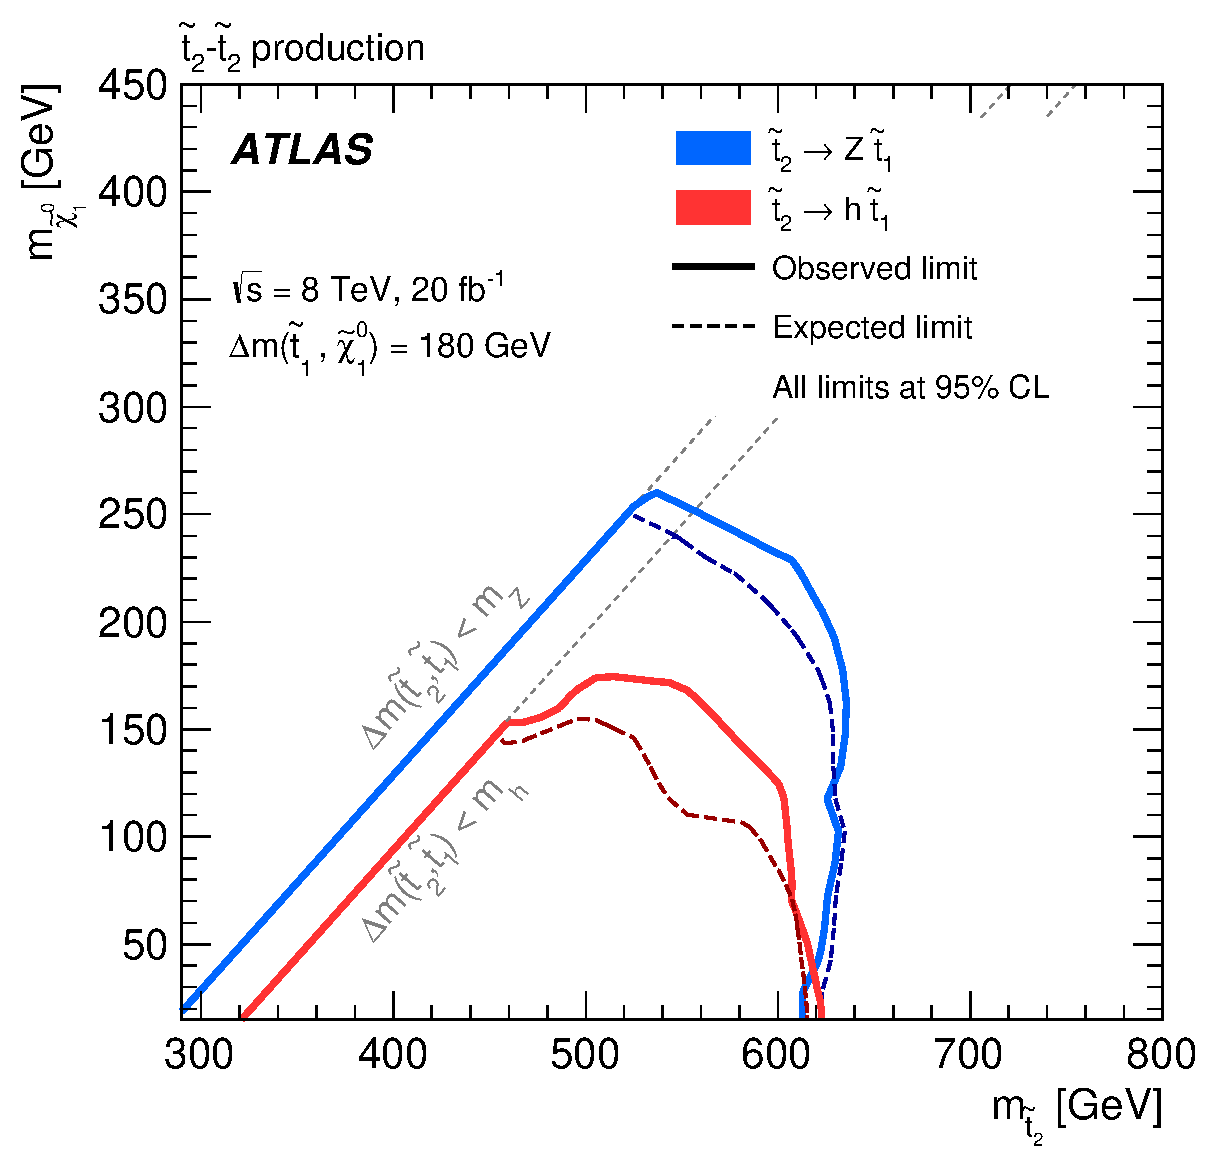
\includegraphics[width=0.6\textwidth]{Analysis/Figures_stop2/lim_2D_stopZ.eps}
\caption{
Expected and observed exclusion limits in the $m_{\st_2}$--$m_{\neut}$ plane for the direct
$\st_2$ pair production simplified model with BR$(\st_2 \to H \st_1)=1$.
The contours of the band around the expected limit are the $\pm 1$ s.d. results, including all uncertainties
except theoretical uncertainties on the signal cross
section. The dotted lines around the observed limit illustrate
the change in the observed limit as the nominal signal cross
section is scaled up and down by the theoretical uncertainty.
All limits are computed at 95\% CL.
\label{fig:lim_2D_stopZ}}
\end{center}
\end{figure}

The analysis presented here has been designed to be sensitive to models with high BR$(\st_2 \to H \st_1)$. Other complementary analyses can be devised targeting the decay channels BR$(\st_2 \to Z \st_1)$ and  BR$(\st_2 \to t \neutralino)$. In particular, traditional third generation squark analyses targeting BR$(\st_1 \to t \neutralino)$ can be easily reinterpreted in the context of BR$(\st_2 \to t \neutralino)$.
ATLAS has published a result in the search for $\stoptwobar$, targeting the decay through a $Z$ boson~\cite{atlas_stop2_Zstop1}.
A combination with this analysis has not been performed but the exclusion limits from both analyses can be overlaid. Figure~\ref{fig:lim_2D_stopZ} shows the corresponding observed and expected limits in the $m_{\st_2}$--$m_{\neut}$ plane. It has to be noted that each analysis assumes a \unit[100]{\%} branching ratio to its decay of interest. A more direct comparison can be performed dropping the branching ratio assumption. Figure~\ref{fig:lim_triangle_stopZ} shows the exclusion limits as a function
of the $\st_2$ branching ratios. A reinterpretation of $\stoponebar$ searches~\cite{Aad:2014bva,Aad:2014kra} is also included to address models with high branching ratio to BR$(\st_2 \to t \neutralino)$.
The three analyses show good complementarity, covering the branching ratio plane and excluding a simplified model with $(m_{\st_2}, m_{\neut}) = (500, 20)\gev$ for any value of the branching ratios.

\begin{figure}[tpb]
\centering
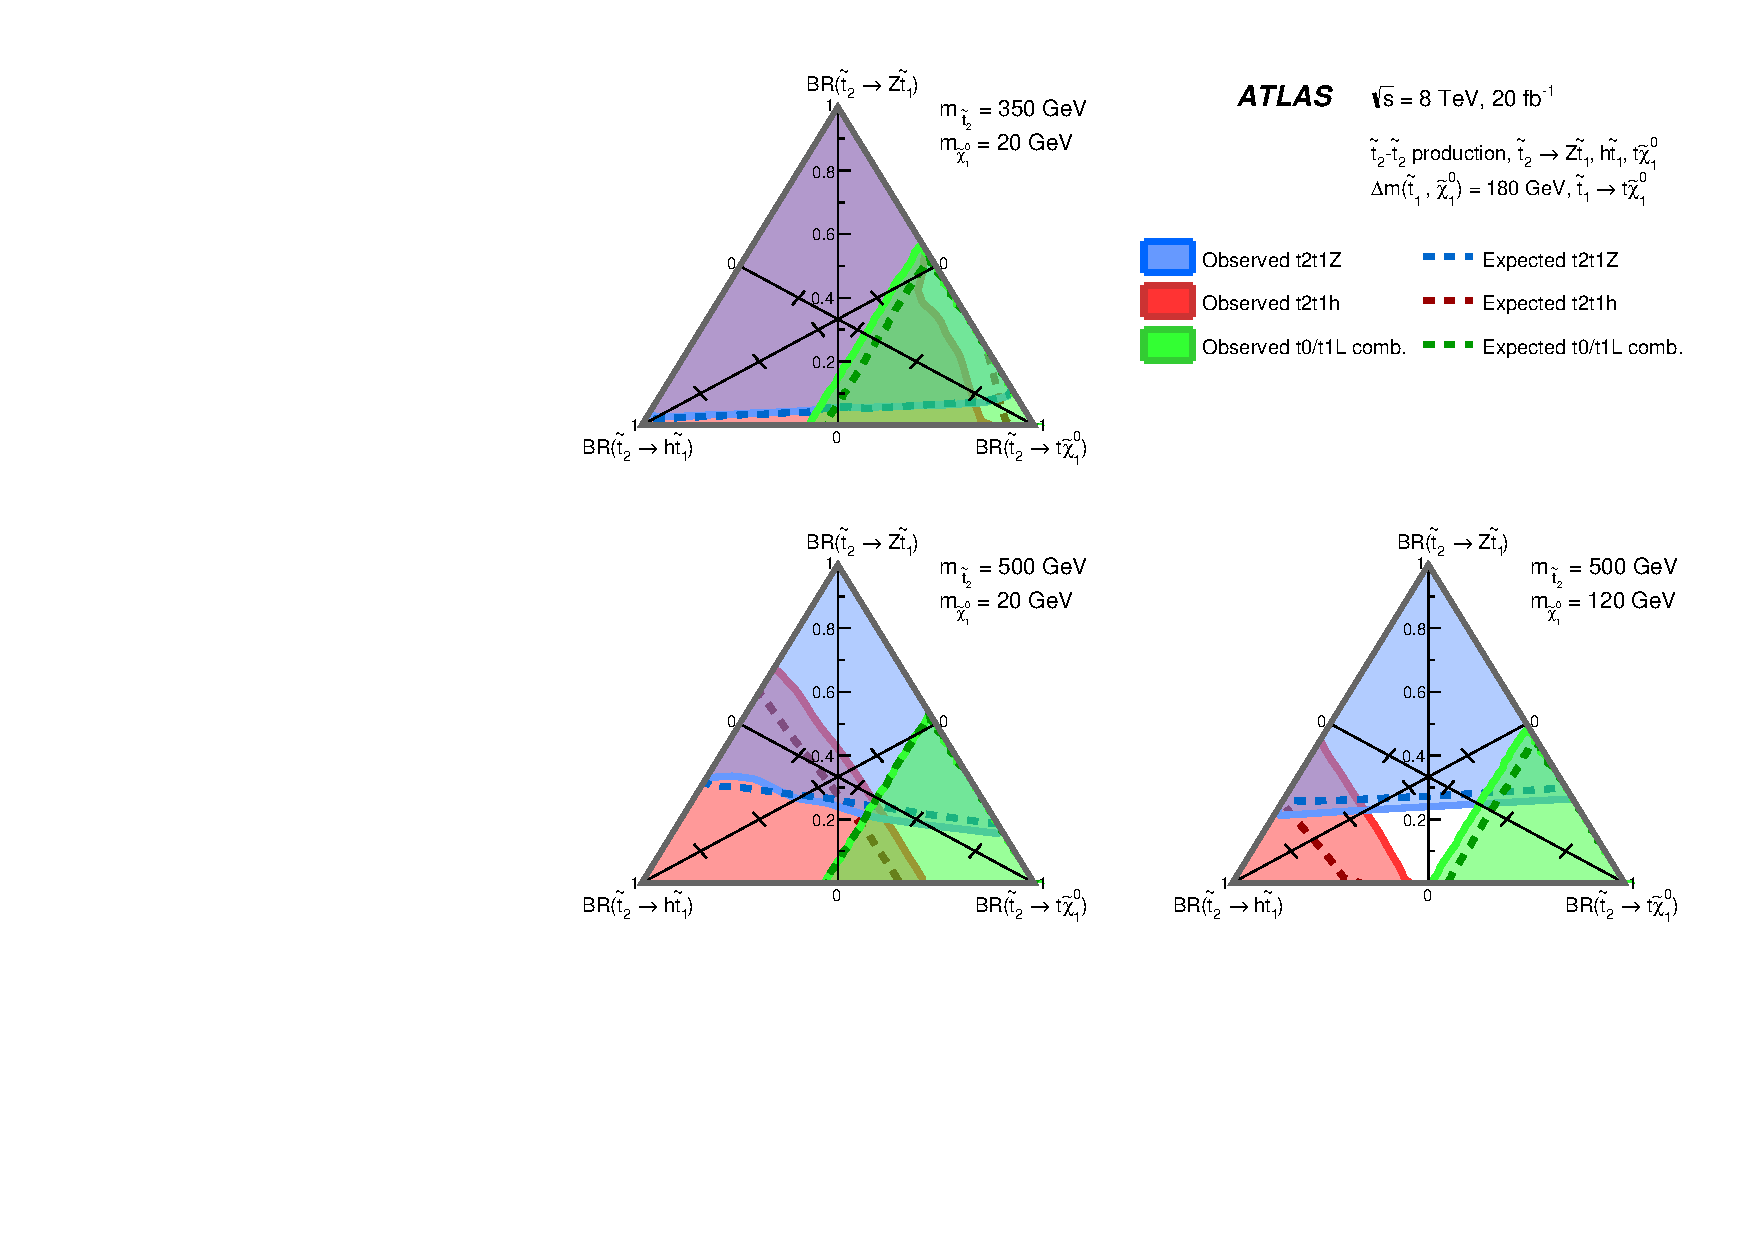
\includegraphics[width=0.9\textwidth]{Analysis/Figures_stop2/lim_triangle_stopZ}
\caption{
Exclusion limits at 95\% CL are shown for the direct $\st_2$ pair production simplified model as a function of the branching
ratios BR$(\st_2 \to Z \st_1)$, BR$(\st_2 \to H \st_1)$ and BR$(\st_2 \to t \neut)$ for (top) $(m_{\st_2}, m_{\neut}) = (350, 20)\gev$,
(bottom left) $(500, 20)\gev$, and (bottom right) $(500, 120)\gev$.
The dashed and solid lines show the expected and observed limits, respectively, including all
uncertainties except the theoretical signal \xsec\ uncertainty (PDF and scale).
\label{fig:lim_triangle_stopZ}}
\end{figure}
